\documentclass[../../note.tex]{subfiles}
\usepackage{authblk}
\begin{document}

% \title{\textbf{Note}}
% \author{Zanqiu Shen}
% \affil{University of Toronto}
% \maketitle

\chapter{Introduction to Quantum Optics}
\section{Introduction}
\begin{itemize}
    \item classicaal: classical atom and light
    \item semiclassical: quantized atom and classical light
    \item quantum mechanical: quantized atom and light
\end{itemize}

\paragraph{Light-Atom Interaction Hamiltonian}
\begin{itemize}
    \item classical dipole in eletric field: dipole moment $\overrightarrow{d} = q \overrightarrow{r}$, $U_I = - \overrightarrow{d} \cdot \overrightarrow{E}$. We have 
    \begin{align}
        \hat{H}_I 
        &= - \hat{d} \cdot \overrightarrow{E}(\overrightarrow{v_0}, t),
    \end{align}
    where $\hat{d} = q \hat{v}$ is the dipole operator.
    \item induced atomic dipole
\end{itemize}

\section{Light Atom Quantum Evolution}
\paragraph{Time Evolution}
We have the Schrodinger equation (both sides) as 
\begin{align}
    i \hbar \frac{\partial}{ \partial t} \vert \Psi(t) \rangle 
    &= (\hat{H}_0 + \hat{H}_I(t))\vert \Psi(t) \rangle,
\end{align}
where the general ansatz (assumption) is 
\begin{align}
    \vert \Psi(t) \rangle
    &= \sum_{n} c_n(t) e^{-i E_n t/\hbar} \vert n \rangle,
\end{align}
and 
\begin{align}
    \hat{H}_0 \vert n \rangle
    &= E_n \vert n \rangle
\end{align}
is the atomic eigenstates. Inserting $\vert \Psi(t) \rangle$ and $\hat{H}_0 \vert n \rangle$ into Schrodinger equation, we get
\begin{align}
    &i \hbar \sum_n \left\{\dot{c}_n e^{-i E_n t/\hbar} \vert n \rangle - \frac{i E_n}{\hbar} c_n e^{-i E_n t/\hbar} \vert n \rangle \right\} 
    = \sum_n \left\{c_n e^{-i E_n t/\hbar} \vert n \rangle + c_n e^{-i E_n t /\hbar} \hat{H}_I \vert n \rangle \right\} \\
    &\Longrightarrow i \hbar \sum_n \dot{c_n}e^{-i E_n t /\hbar} \vert n \rangle = \sum_n c_n e^{-i E_n t /\hbar} \hat{H}_I \vert n \rangle \\
    &\Longrightarrow i \hbar \dot{c_n}e^{-i E_k t /\hbar} \vert= \sum_n c_n(t) e^{-i E_n t/\hbar} \langle k \hat{H}_I(t)\vert n \rangle \\
    &\Longrightarrow i \hbar\dot{c}_k = \sum_n c_n(t) e^{-i E_{n,k} t / \hbar} \langle k \vert \hat{H}_I(t) \vert n \rangle,
\end{align}
where we use
\begin{align}
    \langle k \vert n \rangle 
    &= \delta_{k n}, \\
    E_{n,k}
    &= E_n - E_k, \\
    \omega_{nk}
    &= (E_n - E_k)/\hbar.
\end{align}
and $\langle k \vert \hat{H}_I(t) \vert n \rangle$ is the matrix element.

\section{Time Dependent Perturbation Theory}
Recall the time evolution:
\begin{align}
    i \hbar\dot{c}_k = \sum_n c_n(t) e^{-i \omega_{nk} t} \langle k \vert \hat{H}_I(t) \vert n \rangle,
\end{align}
and
\begin{align}
    \omega_{nk}
    &= (E_n - E_k)/\hbar.
\end{align}

Consider the Simplification (Perturbation Theory)
\begin{itemize}
    \item System only in state $\vert 1 \rangle$ at $t = 0$ $\Longrightarrow c_1 \vert 0 \rangle = 1$ (only the ground state $\vert 1 \rangle$),
    \item Perturbative treatment of interaction term: weak perturbation $\forall \vert c_k(t) \vert^2 <<1$.
\end{itemize}
We then have
\begin{align}
    i \hbar \dot{c}_k
    &= e^{i \omega_{1k}t} \langle k \vert \hat{H}_I(t) \vert 1 \rangle,
\end{align}
with $c_k(0) = 0$, we obtain:
\begin{align}
    c_k(t)
    &= \frac{1}{i \hbar} \int_0^t e^{-i \omega_{1k} t} \langle k \vert \hat{H}_I(t^\prime)\vert 1 \rangle{\rm d}t^\prime.
\end{align}
\begin{example}[Sinusoidal perturbation]
    Define
    \begin{align}
        \hat{H}(t)
        &= \hat{H}_I e^{-i \omega t}.
    \end{align}
    Given the figure in the video, we have
    \begin{align}
        c_k(T)
        &= \frac{1}{i \hbar} \int_{0}^T e^{i \Delta \omega t} \langle k \vert \hat{H}_I \vert 1 \rangle {\rm d}t \\
        &\Longrightarrow Transition~probability~P_{k1}(T) = \vert c_k(T) \vert^2 = \frac{1}{\hbar^2} \vert \langle k \vert \hat{H}_I \vert 1 \rangle \vert^2 Y(\Delta \omega, T),
    \end{align}
    with 
    \begin{align}
        Y(\Delta \omega, T)
        &= \frac{\sin^2(\Delta \omega T/2)}{(\Delta \omega /2)^2} \\
        &\sim {\rm sinc}^2 x,
    \end{align}
    where $\Delta \omega = \omega - \omega_{1 k}$ is the detwining.
\end{example}

Let's take a look at the sinc function $Y(\Delta \omega, T) = {\rm sinc}^2 x$. Transition for $\Delta \omega \leq \frac{2 \pi}{T}$, we have $\Delta \omega \cdot T\leq 2 \pi$, which implies
\begin{align}
    \Delta E \cdot T \leq h,
\end{align}
which is the time-frequency uncertainty. (The expression in the video seems wrong, so I make corrections abrove.) We have the following case
\begin{align}
    \frac{1}{2 \pi T} Y(\Delta \omega, T)
    &\stackrel{T \rightarrow \infty}{\rightarrow} \delta(\Delta \omega),
\end{align}
then we have
\begin{align}
    P_{k1}(T \rightarrow \infty)
    &= \frac{2 \pi}{\hbar^2} \vert \langle k \vert \hat{H}_I \vert i \rangle \vert^2 \delta(\Delta \omega) T.
\end{align}

\paragraph{Fermi's Golden Rule}
$\vert k \rangle$ Quasi continuum of final states. We have the transition probability
\begin{align}
    P_{k1} 
    &= \Gamma_{k1} T,
\end{align}
where
\begin{align}
    \Gamma_{k1}
    &= \frac{2 \pi}{ \hbar} \vert \langle k \vert \hat{H}_I \vert 1 \rangle \vert^2 \rho(E_k = E_1 + \hbar \omega) 
\end{align}
is called the Femi's Golden Rule,
\begin{align}
    \vert \langle k \vert \hat{H}_I \vert 1 \rangle \vert^2
\end{align}
is the coupling strength $\propto E_0^2$ and $\propto I$,
\begin{align}
    \rho(E_k = E_1 + \hbar \omega) 
\end{align}
is the density states which is number of availble final states to the system,
\begin{align}
    \Gamma_{k1}
    &\hat{=} Transition~Rate=\frac{{\rm d}P_{k1}}{{\rm d}T},
\end{align}
and density states
\begin{align}
    \rho(E)
    &= \frac{{\rm d}N}{{\rm d}E},
\end{align}
where $\Delta N$ is the number of states in an energy interval $\Delta E$ around energy $E_k$ and we let $\Delta E$ approaches 0.

\section{Two Level Atom (TLA)}
Given by the figure, in state $\vert 1 \rangle$, we have $E_1 = \hbar \omega_1$ and in state $\vert 2 \rangle$, we have $E_2 = \hbar \omega_2$ and $E_2 - E_1 = \hbar(\omega_2 - \omega_1) = \omega_{21}$. We have the Hamiltonian
\begin{align}
    \hat{H}
    &= \hat{H}_0 - \hat{d} \cdot E(t),
\end{align}
where 
\begin{align}
    E(t)
    &= \varepsilon E_0 \cos(\omega t),
\end{align}
where $\varepsilon$ is the polarization vector, $E_0$ is the field amplitude, and $\omega$ is the frequency of the light field.

\paragraph{Ansatz for Solving TLA}
We have
\begin{align}
    \vert \Psi(t) \rangle
    &= c_1(t) e^{-i \omega_1 t} \vert 1 \rangle +  c_2(t) e^{-i \omega_2 t} \vert 2 \rangle.
\end{align}

\paragraph{Time Evolution Amplitude}
We have
\begin{align}
    \dot{c_1}(t)
    &= i \frac{d^{\varepsilon}_{12} E_0}{\hbar} e^{- \omega_{21}} \cos(\omega t)c_2(t) \\
    \dot{c_2}(t)
    &= i \frac{d^{\varepsilon}_{12} E_0}{\hbar} e^{+ \omega_{21}} \cos(\omega t)c_1(t),
\end{align}
where 
\begin{align}
    d^{\varepsilon}_{12} 
    &= \langle 1 \vert \hat{d} \cdot \varepsilon \vert 2 \rangle \\
    &= \langle 1 \vert \hat{d} \vert 2 \rangle \cdot \varepsilon \\
    &= \langle 1 \vert \hat{d}_x \vert 2 \rangle \cdot \varepsilon_x +\langle 1 \vert \hat{d}_y \vert 2 \rangle \cdot \varepsilon_y + \langle 1 \vert \hat{d}_z \vert 2 \rangle \cdot \varepsilon_z.
\end{align}
is the Dipole Matrix Element, which is the atomic property and we assume it's real. We also define
\begin{align}
    \Omega_0
    &= \frac{d_{12}^{\varepsilon} E_0}{\hbar}
\end{align}
as the Rubi frequency.

\paragraph{Time Evolution}
Using Euler' form, we have
\begin{align}
    \dot{c_1}(t)
    &= i \frac{\Omega_0}{2} e^{- \omega_{21}} (e^{i \omega t} + e^{-i \omega t})c_2(t) \\
    \dot{c_2}(t)
    &= i \frac{\Omega_0}{2} e^{+ \omega_{21}} (e^{i \omega t} + e^{-i \omega t}) c_1(t)
\end{align}
by
\begin{align}
    \cos \alpha
    &= \frac{1}{2} (e^{i \alpha} + e^{-i \alpha})
\end{align}
and
\begin{align}
    e^{i \alpha}
    &= \cos \alpha + i \sin \alpha.
\end{align}

\paragraph{Rotating Wave Approximation}
We have
\begin{align}
    \dot{c_1}(t)
    &= i \frac{\Omega_0}{2}  (e^{+ i (\omega - \omega_{21}) t} + e^{-i (\omega + \omega_{21}) t})c_2(t) \\
    \dot{c_2}(t)
    &= i \frac{\Omega_0}{2}  (e^{- i (\omega - \omega_{21}) t} + e^{+i (\omega + \omega_{21}) t}) c_1(t),
\end{align}
and we ignore the sum frequency term and get
\begin{align}
    \dot{c_1}(t)
    &= i \frac{\Omega_0}{2}  e^{+ i (\omega - \omega_{21}) t} c_2(t) \\
    \dot{c_2}(t)
    &= i \frac{\Omega_0}{2}  e^{- i (\omega - \omega_{21}) t}  c_1(t),
\end{align}
which is a good approcimation for detwining $\delta = \omega - \omega_{21} \approx 0$.
We introduce
\begin{align}
    \tilde{c_1}(t)
    &= c_1(t) e^{-i \frac{\delta}{2} t} \\
    \tilde{c_2}(t)
    &= c_2(t) e^{+i \frac{\delta}{2} t}. \\
\end{align}
\paragraph{Ansatz Wavefunctions for TLA}
Whole time evolution in state amplitudes
\begin{align}
    \vert \Psi(t) \rangle 
    &= c_1^\prime(t) \vert 1 \rangle + c_2^\prime(t) \vert 2 \rangle.
\end{align}
Time evolution when field is off
\begin{align}
    \vert \Psi(t) \rangle 
    &= c_1^\prime(0) e^{-i \omega_1 t} \vert 1 \rangle + c_2^\prime(0) e^{-i \omega_2} \vert 2 \rangle.
\end{align}
However, this is boring. We chose different ansatz as
\begin{align}
    \vert \Psi(t) \rangle
    &= c_1(t) e^{-i\omega_1 t} \vert 1 \rangle + c_2(t) e^{-i\omega_2 t} \vert 2 \rangle \\
    &\Longleftrightarrow \vert \Psi(t) \rangle
    = c_1(t)  \vert 1 \rangle + c_2(t) e^{-i\omega_{21} t} \vert 2 \rangle, 
\end{align}
where $c_1(t)$ and $c_2(t)$ capture time evolution on top of eigenstate evolution! We now have
\begin{align}
    \vert \Psi(t) \rangle
    &= c_1(t)  \vert 1 \rangle + c_2(t) e^{-i\omega_{21} t} \vert 2 \rangle,
\end{align}
which is called the rotating frame of atom. We also have Rotating frame of light field as
\begin{align}
    \vert \Psi(t) \rangle
    &= \tilde{c_1}(t)  \vert 1 \rangle + \tilde{c_2}(t) e^{-i\omega t} \vert 2 \rangle,
\end{align}
where $\omega$ is the light frequency, $\tilde{c_1}$ and $\tilde{c_2}$ describe time evolution on top of fast light field oscilation.

\paragraph{Solving the TLA Dynamics}
We have the following equations:
\begin{align}
    \frac{d}{d t} \left(\begin{matrix}
        \tilde{c_1}(t) \\
        \tilde{c_2}(t)
    \end{matrix}\right) =  \frac{i}{2} \left(\begin{matrix}
        -\delta & \Omega_0 \\
        \Omega_0 & + \delta
    \end{matrix}\right) \left(\begin{matrix}
        \tilde{c_1}(t) \\
        \tilde{c_2}(t)
    \end{matrix}\right).
\end{align}
Considering the simplest case $\delta = 0$
\begin{align}
    \frac{d}{d t} \tilde{c_1}(t)
    &= \frac{i}{2} \Omega_0 \tilde{c_2}(t) \\
    \frac{d}{d t} \tilde{c_2}(t)
    &= \frac{i}{2} \Omega_0 \tilde{c_1}(t).
\end{align}
Take time dirivative of the first equation, then we have
\begin{align}
    \ddot{c_1}(t)
    &= - \frac{\Omega_0^2}{4} \tilde{c_1}(t),
\end{align}
the solutions of which are
\begin{align}
    \tilde{c_1}(t) = \cos(\Omega_0 t/2) \\
    \tilde{c_2}(t) = i \sin(\Omega_0 t/2)
\end{align}
for $\tilde{c_1}(0) = 1$ and $\tilde{c_2}(0) = 0$. Also we can obtain the excited state probability as
\begin{align}
    P_2(t)
    &= \vert c_2(t) \vert^2 \\
    &= \vert \tilde{c_2}(t) \vert^2.
\end{align}

\paragraph{Rabi Oscillations (Resonant Case)}
Nonlinear Response can be seen from the figure.

\paragraph{General Rabi Oscillations (with detuning)}
Given the figurem.
\begin{align}
    \vert \tilde{c_2}(t) \vert^2
    &= \frac{\Omega_0^2}{\Omega} \sin^2\left(\frac{1}{2}\Omega t\right) \\
    &= \frac{\Omega_0^2}{2 \Omega^2} \left\{1-\cos(\Omega t)\right\},
\end{align}
where $\Omega = \sqrt{\Omega_0^2 + \delta^2}$ is the effective Rabi frequency.

\paragraph{Interesting Special Cases}
a) Pi-Puls $\Omega_0 \tau = \pi$: swap population 
\begin{align}
    \vert 1 \rangle \rightarrow i \vert 2 \rangle \\
    \vert 2 \rangle \rightarrow i \vert 1 \rangle.
\end{align}

b) 2Pi-Puls $\Omega_0 \tau = 2 \pi$: flip the sign

c) Pi/2-Puls $\Omega_0 \tau = \pi/2$: superposition state

\section{Oscillating Dipoles}
\paragraph{Atomic Eigenstates}
\begin{align}
    \vert \Psi_{nlm}(t) \rangle 
    &= e^{-i E_{nlm} t/\hbar} \vert \Psi_{nlm}(0) \rangle, \\
    \hat{H_0} \vert \Psi_{nlm}(0) \rangle
    &= E_{nlm} \vert \Psi_{nlm} \rangle,
\end{align}
and the electron density is
\begin{align}
    \rho(r, \theta, \phi)
    &= \vert \Psi(r, \theta, \phi, t = 0)^2 \vert.
\end{align}

\paragraph{Atomic Dipole}
Calculate (Oscillating) Dipole Moment for Atomic Eigenstate. We denote 
$\vert 1 \rangle = \vert \Psi_{nlm} \rangle$. We have
\begin{align}
    d(t)
    &= \langle 1(t) \vert \hat{d} \vert 1(t) \rangle \\
    &= \langle \hat{d} \vert 1 \rangle \\
    &= -e \langle 1 \vert \hat{r} \vert 1 \rangle.
\end{align}
Then, 
\begin{align}
    -e \langle 1 \vert \hat{r} \vert 1 \rangle 
    &= -e \langle 1 \vert \hat{P} \hat{P}^{-1} \hat{r} \hat{P} \hat{P}^{-1} \vert 1 \rangle \\
    &= + e \langle 1 \vert \hat{r} \vert 1 \rangle,
\end{align}
which implies
\begin{align}
    \langle 1 \vert \hat{r} \vert 1 \rangle 
    &= 0.
\end{align}

\paragraph{Atomic Dipole - Superposition States}
Calculate (Oscillating) Dipole Moment for Atomic Superposition State 
\begin{align}
    \vert \Psi(0) \rangle
    &= \frac{1}{\sqrt{2}}(\vert 1 \rangle + i \vert 2 \rangle).
\end{align}
Evolution
\begin{align}
    \vert \Psi(t) \rangle
    &= \frac{1}{\sqrt{2}}(\vert 1 \rangle + i e^{- i \omega_{21} t} \vert 2 \rangle).
\end{align}
We have
\begin{align}
    d(t)
    &= \langle \Psi(t) \vert \hat{d} \vert \Psi(t) \rangle \\
    &= \frac{1}{2}\left\{\langle 1 \vert \hat{d} \vert 1 \rangle + \langle 2 \vert \hat{d} \vert 2 \rangle + i e^{-i\omega_{21} t} \langle 1 \vert \hat{d} \vert 2 \rangle - i e^{-i\omega_{21} t} \langle 2 \vert \hat{d} \vert 1 \rangle\right\} \\
    &= d_{12} i \frac{1}{2} \left\{e^{-i \omega_{21} t} - e^{i \omega_{21} t}\right\} \\
    &= d_{12} \sin(\omega_{21} t),
\end{align}
where $d_{12}$ is the dipole moment amplitude, $\omega_{21}$ is the natural resonance frequency.

\paragraph{Electron Density - Superposition States}
Calculate Electron Probability Density for Superposition State. The superposition state is
\begin{align}
    \Psi(r,t)
    &= \frac{1}{\sqrt{2}} \left(\Psi_1(r) + i e^{-i \omega_{21} t} \Psi_2D(t) \right).
\end{align}
The Electron Probability Density is
\begin{align}
    \rho(r, t)
    &= \vert \Psi(r, t) \vert^2 \\
    &= \Psi^\ast \Psi \\
    &= \frac{1}{2} \left\{\vert \Psi_1(r) \vert^2 + \vert \Psi_2(r) \vert^2 + 2{\rm Re}\left(i e^{-i \omega_{21} t} \Psi_1^*(r) \Psi_2(r)\right)\right\},
\end{align}
where $2{\rm Re}\left(i e^{-i \omega_{21} t} \Psi_1^*(r) \Psi_2(r)\right)$ is the interference term.

\paragraph{Examples}
This is shown by animation and figure in the video.



\section{The Bloch Sphere}
\paragraph{General Two-Level State}
\begin{itemize}
    \item General State Description
    \begin{align}
        \vert \Psi \rangle
        &= c_1^\prime \vert 1 \rangle + c_2^\prime \vert 2 \rangle \\
        &\qquad\eqnote{Up to a global phase} \\
        &= \vert c_1^\prime \vert \vert 1 \rangle + e^{i \phi} \vert c_2^\prime \vert 2 \rangle
    \end{align}
    satisfying $\vert c_1^\prime \vert^2 + \vert c_2^\prime \vert^2 = 1$.
    \item Alternative way
    \begin{align}
        \vert \Psi \rangle
        &= \cos(\theta/2) \vert 1 \rangle + e^{i \phi} \sin(\theta/2) \vert 2 \rangle,
    \end{align}
    since $\cos(\theta/2)^2 + \sin(\theta/2)^2 = 1$.
\end{itemize}

\paragraph{Geometric Description - Bloch Sphere}
We then have
\begin{align}
    \vert \Psi \rangle
    &= \cos(\theta/2) \vert 1 \rangle + e^{i \phi} \sin(\theta/2) \vert 2 \rangle
\end{align}
with $0 \leq \theta \leq \pi$ as the latitude and $0 \leq \phi \leq 2 \pi$ as the longitude. This is the Bloch Sphere representation. The definition of $\theta$ and $\theta$ and their ranges are different from my familiar coordinate system.

\paragraph{Special States on Bloch Sphere}

\paragraph{Analogy to Spin -1/2 States}
Is is shown in the figure.

\section{Density Operator and Density Matrix}
\paragraph{The Problem}
How do we describe "imperfect state preparation" in an experiment? For example, $50 \% \vert 1 \rangle$ and $50 \% \vert 2 \rangle$. We may think of 
\begin{align}
    \vert \Psi \rangle 
    &= \frac{1}{\sqrt{2}} \left(\vert 1 \rangle + \vert 2 \rangle \right). ???
\end{align}
This is $100 \% \vert \Psi \rangle$ pure state. We need stable relative phase between the two states!

\paragraph{Optical Analogy - Controlled Phase}
The double slit problem is shown in the video.

Intensity on Detection Screen:
\begin{align}
    I 
    &\propto \vert E \vert^2 = \vert E_1 + e^{i \phi} E_2 \vert^2 \\
    &= \vert E_1 \vert^2 + \vert E_2 \vert^2 + 2 {\rm Re}\left(E_1 E_2 e^{i \phi}\right).
\end{align}
As $\phi$ varies, Interference pattern "washed out"!

We need new formalism to describe mixed states!(imperfect state preparation, spontaneous emission,\dots)

\paragraph{Density Operator and Matrix}
The description of mixed states can be handled by the density operator (matrix) formalism!

\begin{itemize}
    \item Density operator (hermitian)
    \begin{align}
        \hat{\rho}
        &= \sum p_i \vert \Psi_i \rangle \langle \Psi_i \vert \\
        \hat{\rho}
        &= I \hat{\rho} I \\
        &= \sum_{i,j} \vert i \rangle \langle i \vert \hat{\rho} \vert j \rangle \langle j \vert \\
        &= \rho_{11} \vert 1 \rangle \langle  1 \vert + \rho_{12} \vert 1 \rangle \langle 2 \vert + \rho_{21} \vert 2 \rangle \langle 1 \vert + \rho_{22} \vert 2 \rangle \langle 2 \vert,
    \end{align}
    where $I = \sum_i \vert i \rangle \langle i \vert$.
    \item Density matrix
    \begin{align}
        \rho
        &= \left[\begin{matrix}
            \rho_{11} & \rho_{12} \\
            \rho_{21} & \rho_{22}
        \end{matrix}\right],
    \end{align}
    where $\rho_{11}$ and $\rho_{22}$ are the populations, $\rho_{12}$ and $\rho_{21}$ are the coherence. Since $\rho$ is hermitian, we have
    \begin{align}
        \rho_{12}
        &= \rho_{21}^\ast.
    \end{align}
\end{itemize}

\begin{example}[Example: Density Matrix of Pure State]
    We have
    \begin{align}
        \vert \Psi \rangle
        &= \vert c_1 \vert \vert 1 \rangle + e^{i \phi} \vert c_2 \vert \vert 2 \rangle.
    \end{align}
    The corresponding density operator of the \textbf{pure state} is $\hat{\rho} = \vert \Psi \rangle \langle \Psi \vert$. Then the corresponding density matrix is 
    \begin{align}
        \rho
        &= \left[\begin{matrix}
            \vert c_1 \vert^2 & \vert c_1 \vert \vert c_2 \vert e^{-i \phi} \\
            \vert c_1 \vert \vert c_2 \vert e^{i \phi} & \vert c_2 \vert^2
        \end{matrix}\right],
    \end{align}
    where $\vert c_1 \vert \vert c_2 \vert e^{-i \phi}$ and $\vert c_1 \vert \vert c_2 \vert e^{i \phi}$ are relative phase between states $\vert 1 \rangle$ and $\vert 2 \rangle$.

    specific example:
    \begin{align}
        \vert \Psi \rangle
        &= \frac{1}{\sqrt{2}} \left(\vert 1 \rangle + \vert 2 \rangle \right),
    \end{align}
    so
    \begin{align}
        \rho
        &= \left[
        \begin{matrix}
            1/2 & 1/2 \\
            1/2 & 1/2
        \end{matrix}
        \right].
    \end{align}
\end{example}

\begin{example}[Example: Fully Incoherent Mixture]
    \begin{align}
        \hat{\rho}
        &= \frac{1}{2} \vert 1 \rangle \langle 1 \vert + \frac{1}{2} \vert 2 \rangle \langle 2 \vert
    \end{align}
    with 
    \begin{align}
        \rho
        &= \left[\begin{matrix}
            1/2 & 0 \\
            0 & 1/2
        \end{matrix}\right],
    \end{align}
    where vanishingly coherence and the phase varies from $0$ to $2 \pi$. It means that we did not control phase.
\end{example}

\paragraph{Useful Facts}
\begin{itemize}
    \item Expectation values: $\langle \hat{A} \rangle = \tr(\hat{\rho} \hat{A}) = \tr(\rho A)$
    \item Time evolution (von Neumann equation)
    \begin{align}
        i \hbar \frac{\partial \hat{\rho}}{\partial t} 
        &= [\hat{H}, \hat{\rho}]
    \end{align}
    \item Pure state:  $\tr(\rho^2) = 1$
    \item Mixed states: $\tr(\rho^2) < 1$
\end{itemize}

\section{Optical Bloch Equations}
\paragraph{Time Evolution of Density Matrix}
How to calculate time evolution of density matrix?
\begin{align}
    i \hat{\hbar} \frac{\partial \hat{\rho}}{\partial t}
    &= [\hat{H}, \hat{\rho}].
\end{align}
Assume pure state
\begin{align}
    \frac{d}{d t} \rho_{11}
    &= \frac{d}{d t}(c_1 c_1^\ast) \\
    &= \dot{c}_1 c_1^\ast + c_1 \dot{c}_1^\ast \\
    &= i \frac{\Omega_0}{2} \left(e^{i \delta t} \rho_{21} - e^{-i \delta t} \rho_{12} \right) \\
    &\qquad\eqnote{Transformation to rotality frame of light} \nonumber \\
    &= i \frac{\Omega_0}{2} \left(\tilde{\rho}_{21} - \tilde{\rho}_{12}\right),
\end{align}
where
\begin{align}
    \dot{c}_1(t)
    &= i \frac{\Omega_0}{2} e^{+i \delta t} c_2(t) \\
    \dot{c}_2(t)
    &= i \frac{\Omega_0}{2} e^{-i \delta t} c_1(t) \\
    \tilde{\rho}_{12} 
    &= e^{-i \delta t} \rho_{12} \\
    \tilde{\rho}_{21} 
    &= e^{+i \delta t} \rho_{21}.
\end{align}
Other elements obtained in analogy!
\begin{align}
    \frac{d}{d t} \rho_{11}
    &= i \frac{\Omega_0}{2} \left(\tilde{\rho}_{21} - \tilde{\rho}_{12}\right) \\
    \frac{d}{d t} \rho_{22}
    &= i \frac{\Omega_0}{2} \left(\tilde{\rho}_{12} - \tilde{\rho}_{21}\right) \\
    \frac{d}{d t} \tilde{\rho}_{12}
    &= -i \delta \tilde{\rho}_{12} + i \frac{\Omega_0}{2} \left(\rho_{22} - \rho_{11}\right) \\
    \frac{d}{d t} \tilde{\rho}_{21}
    &= +i \delta \tilde{\rho}_{21} + i \frac{\Omega_0}{2} \left(\rho_{11} - \rho_{22}\right).
\end{align}
Noting that $\tilde{\rho}_{12} = \tilde{\rho}_{21}$ due to hermitian matrix, the third and the forth equations are the same. So we have
\begin{align}
    \frac{d}{d t} \rho_{11}
    &= i \frac{\Omega_0}{2} \left(\tilde{\rho}_{21} - \tilde{\rho}_{12}\right) \\
    \frac{d}{d t} \rho_{22}
    &= i \frac{\Omega_0}{2} \left(\tilde{\rho}_{12} - \tilde{\rho}_{21}\right) \\
    \frac{d}{d t} \tilde{\rho}_{12}
    &= -i \delta \tilde{\rho}_{12} + i \frac{\Omega_0}{2} \left(\rho_{22} - \rho_{11}\right).
\end{align}
\paragraph{Optical Bloch Equations with Damping}
Phenomenological damping and spontaneous emission in the figure. Combine the decay, we have
\begin{align}
    \frac{d}{d t} \rho_{11}
    &= i \frac{\Omega_0}{2} \left(\tilde{\rho}_{21} - \tilde{\rho}_{12}\right) + \gamma \rho_{22} \\
    \frac{d}{d t} \rho_{22}
    &= i \frac{\Omega_0}{2} \left(\tilde{\rho}_{12} - \tilde{\rho}_{21}\right) -\gamma \rho_{22}\\
    \frac{d}{d t} \tilde{\rho}_{12}
    &= -i \delta \tilde{\rho}_{12} + i \frac{\Omega_0}{2} \left(\rho_{22} - \rho_{11}\right) - (\gamma/2)\tilde{\rho}_{12}.
\end{align}
We now define the inversion $w = \rho_{22} - \rho_{11}$. We have Optical Bloch Equations with Damping
\begin{align}
    \frac{d}{d t} \tilde{\rho}_{21}
    &= -\left(\gamma/2 - i \delta \right) \tilde{\rho}_{21} - \frac{i \omega \Omega_0}{2} \\
    \frac{d}{d t}\omega
    &= -\gamma \left(\omega + 1\right) - i \Omega_0 \left(\tilde{\rho}_{21} - \tilde{\rho}_{12}\right)
\end{align}
in the Density Matrix Form.

\section{Optical Bloch Equations - Dynamics and Steady State}
\paragraph{Dynamical Evolution of System}
Shown in the figure in the picture.

\paragraph{Steady State Solution}
Conditions: $\frac{d}{d t} \tilde{\rho}_{21} = 0$ and $\frac{d}{d t}\omega = 0$. Then we have the solutions
\begin{align}
    \omega
    &= - \frac{1}{1 + S} \\
    \tilde{\rho}_{21}
    &= \frac{2 \Omega_0}{2\left(\gamma/2 - -\delta \right)\left(1+S\right)} \\
    S
    &= \frac{\Omega_0^2/2}{\delta^2 + \gamma^2/4} = \frac{S_0}{1+4 \delta^2/\gamma^2} \\
    S_0
    &= \frac{2 \Omega_0^2}{\gamma^2} = \frac{I}{O_{sat}},
\end{align}
where $S$ is called the saturation parameter, $S_0$ is called resonant saturation parameter.

Limiting Cases: 
\begin{itemize}
    \item $S \leq \leq 1$: $w \rightarrow -1$ where $w = \rho_{22} - \rho_{11}$. Atom is mainly in ground state.
    \item $S \geq\geq 1$: $S \rightarrow \infty$, $w \rightarrow 0$.
\end{itemize}

\begin{itemize}
    \item Excited State Population: 
    \begin{align}
        \rho_{22} \\
        &\qquad\eqnote{Combine with $\rho_{22} + \rho_{11} = 1$} \nonumber \\
        &= \frac{1}{2} (1+w) \\
        &= \frac{S}{2(1+S)} \\
        &= \frac{S_0/2}{1+S_0+4 \delta^2/\gamma^2} \\
        &\stackrel{S_0 \rightarrow \infty, \delta = 0}{\longrightarrow} \frac{1}{2}.
    \end{align}
    \item Photon Scattering Rate: $\Gamma_{ph} = \gamma \rho_{22} = \frac{\gamma}{2} \frac{S_0}{1+S_0+4 \delta^2/\gamma^2}$. $\Gamma_{ph} \rightarrow \gamma/2$ for $S_0 \rightarrow \infty$ and $\delta = 0$. We rewrite it as
    \begin{align}
        \Gamma_{ph}
        &= \left(\frac{S_0}{1+S_0}\right)\left(\frac{\gamma/2}{1+4 \delta^2 / \gamma'^2}\right) \\
        \gamma'
        &= \gamma \sqrt{1+S_0}.
    \end{align} 
\end{itemize}
It has a figure in the video. The saturation brodening is shown in the figure.

\section{Lambert-Beer Law}
\paragraph{Attenuation of Light}
It is shown in the figure.

\paragraph{Scattered Light from Slab of Atoms}
scattered light power by slab of length $d z$
\begin{align}
    d P_{sc}
    &= \Gamma_{ph} \times n A dz \times \hbar \omega,
\end{align}
where $\Gamma_{ph}$ is the single atom photon scattering rate, $\hbar \omega$ is the energy of single atom, $n A d z$ is the number of atoms. Then we have
\begin{align}
    \frac{d P_{sc}}{d z}
    &= \Gamma_{ph} \times nA \times \hbar \omega.
\end{align}

\paragraph{Scattered Light from Slab of Atoms}
Energy conservation requires
\begin{align}
    \frac{d P}{d z}
    &= - \frac{d P_{sc}}{d z} \\
    \frac{d P}{d z}
    &= \frac{d I}{d I} A.
\end{align}

Put every thing together:
\begin{align}
    \frac{d I}{d z}
    &= -\Gamma n \hbar \omega.
\end{align}
We have
\begin{align}
    \frac{d I(z)}{d z}
    &= - n \sigma I(z),
\end{align}
where $\sigma$ is the atomic scattering cross section.

\paragraph{Lambert-Beer Law (no saturation)}
We compute the solutions
\begin{align}
    I(z)
    &= I(0)e^{-n \sigma z},
\end{align}
which is the Lambert-Beer Law of Absorption.

\paragraph{Laser induced Fluorescence}
Shown in a video.

\section{Bloch Vector}
\paragraph{Density Matrix Revisited}
Density Matrix of TLA
\begin{align}
    \rho
    &= \left(\begin{matrix}
        \rho_{11} & \rho_{12} \\
        \rho_{21} & \rho_{22}
    \end{matrix}\right)
\end{align}

Density Matrix hermitian
\begin{align}
    \rho
    &= \rho^\dagger = (\rho^T)^\ast,
\end{align}
so we have
\begin{align}
    \rho
    &= \left(\begin{matrix}
        \rho_{11} & {\rm Re}\rho_{12} + i {\rm Im}\rho_{12} \\
        {\rm Re}\rho_{12} - i {\rm Im}\rho_{12} & \rho_{22}
    \end{matrix}\right).
\end{align}

Pauli matrices are
\begin{align}
    \sigma_x
    &= \left(\begin{matrix}
        0 & 1\\
        1 & 0
    \end{matrix}\right)
    \sigma_y
    = \left(\begin{matrix}
        0 & -i\\
        i & 0
    \end{matrix}\right)
    \sigma_x
    = \left(\begin{matrix}
        1 & 0\\
        0 & -1
    \end{matrix}\right).
\end{align}
The decomposition of Density matrix into Pauli matrices
\begin{align}
    \rho
    &= \frac{1}{2}\left(I + b_x \sigma_x + b_y \sigma_y + b_z \sigma_z \right),
\end{align}
where $b_x, b_y,b_y \in \mathbb{R}$.

\paragraph{Bloch Vector}
We have the density matrix in rotating frame of light
\begin{align}
    \tilde{\rho}
    &= \left(\begin{matrix}
        \rho_{11} & \tilde{\rho}_{12} \\
        \tilde{\rho}_{21} & \rho_{22}
    \end{matrix}\right),
\end{align}
where $\tilde{\rho}_{12} = \rho_{12} e^{-i \omega t}$. We use following sign convention and have
\begin{align}
    \tilde{\rho}
    &= \frac{1}{2} \left(I + u \sigma_x - v \sigma_y - w \sigma_z \right),
\end{align}
and the bloch vector is defined as
\begin{align}
    \left(\begin{matrix}
        u \\
        v \\
        w
    \end{matrix}\right).
\end{align}
It can be easily shown that
\begin{align}
    u
    &= 2 {\rm Re}(\tilde{\rho}_{12}) = \tilde{\rho}_{12} + \tilde{\rho}_{12}^\ast \\
    v
    &= 2 {\rm Im}(\tilde{\rho}_{12}) = i (\tilde{\rho}_{12}^\ast + \tilde{\rho}_{12}) \\
    w
    &= \rho_{22} - \rho_{11}, \\
\end{align}
where $u$ is the dispersive component, $v$ is the absorption component and $w$ is the inversion.

Bloch vector can be used to describe any state of TLA density matrix!

Properties of Bloch Vector
\begin{itemize}
    \item Mixed State: $u^2 + v^2 +w^2 < 1 $
    \item Pure State: $u^2 + v^2 +w^2 = 1 $
\end{itemize}

\section{Understanding Bloch Vector}
What physical behaviour do the components stand for?

\begin{itemize}
    \item $w=-1$ atom in ground state. $w = +1$ atom in excited state.
    \item What about $u,v$?
    \begin{align}
        \langle \hat{d}_i(t)
        &= \tr(\hat{\rho} \hat{d}) \\
        &= \tr\left[\left(\begin{matrix}
            \rho_{11} & \rho_{12} \\
            \rho_{12}^\ast & \rho_{22} 
        \end{matrix}\right) \left(\begin{matrix}
            0 & d_{12}^i \\
            d_{12}^i & 0
        \end{matrix}\right)\right],
    \end{align}
    where $d_{12}^x = \langle 1 \vert -q \hat{x} \vert 2 \rangle$.

    Written in the vector form, we have
    \begin{align}
        \langle \hat{d}  \rangle(t)
        &= d_{12} \left(\rho_{12} + \rho_{12}^\ast \right) \\
        &= d_{12} \left(\tilde{\rho}_{12} e^{i \omega t} + \tilde{\rho}_{12}^\ast e^{-i \omega t}\right) \\
        &= d_{12} \left[u\cos(\omega t) - v \sin(\omega t) \right],
    \end{align}
    where we use $\rho_{12} = \tilde{\rho}_{12} e^{i \omega t}$, $u$ denotes in phase and $v$ denotes $90^\circ$ out of phase component.

    Reminder: $E(t) = \epsilon E_0 \cos(\omega t)$.
    \item Which component responsible for absorption/emission? We have a figure in the video to show the classical picture.
    
    Average absorbed power per atom (classical ensemble average)
    \begin{align}
        \langle \frac{d W}{d t} 
        &= \epsilon E_0 \cos(\omega t)\langle -q \frac{d r}{d t} \rangle \\
        &= \epsilon E_0 \cos(\omega t) \langle \dot{d} \rangle.
    \end{align}

    Quantum mechanical analogue (Ehrenfest)
    \begin{align}
        \langle \frac{d W}{d t} \rangle
        &= \epsilon E_0 \cos(\omega t) \langle \dot{d} \rangle \\
        \langle \hat{d} \rangle(t)
        &= d_{12} [u \cos(\omega t) - v \sin(\omega t)]. \\
        \langle \frac{d W}{d t} \rangle
        &= -d_{12} \cdot \epsilon E_0 \omega (u \cos(\omega t) \sin(\omega t) + v \sin(\omega t)^2) \\
        \overline{\langle \frac{d W}{d t} \rangle}
        &= \frac{1}{T} \int dt \langle \frac{d W}{d t} \rangle \\
        &= - \frac{d_{12} \cdot \epsilon E_0 \omega v}{2} \\
        &= - \hbar \frac{d_{12} \epsilon E_0}{\hbar} \omega \frac{v}{2} \\
        &= - \hbar \Omega_0 \omega \frac{v}{2},
    \end{align}
    which is the absorption.
\end{itemize}

\section{Optical Bloch Equations using Bloch Vector}


\section{Interlude: The Mach-Zehnder Interferometer}

\section{Ramsey Interferometer}

\section{Review: QM of the Harmonic Oscillator}
\SZQ{2023.04.20: I have understandard the content in this video.}

\section{Wave equation and energy density of classical radiation field}
This section  is also known as the review of Maxwell equations vector potentials.

\paragraph{Fundamentaals}
Maxwell equations in free space
\begin{align}
    \label{eq: Maxwell equations in free space}
    &\nabla \cdot E = 0, \nabla \times E = - \frac{\partial B}{\partial t} \\
    &\nabla \cdot B = 0, \nabla \times B = \frac{1}{c^2} \frac{\partial E}{\partial t}.
\end{align}

\begin{lemma}[Coulomb Gauge]
    \label{lemma: Coulomb Gauge}
    Considering Coulomb Gauge, we have
    \begin{align}
        \nabla \cdot A = 0.
    \end{align}
    Then we can express the eletric field and magnetic field in terms of the vector potential 
    \begin{align}
        & B(r,t) = \nabla \times A(r,t) \\
        & E(r,t) = -\frac{\partial A(r,t)}{\partial t}.
    \end{align}
\end{lemma}

\begin{lemma}[Wave equation]
    \label{lemma: wave equation}
    Considering Coulomb Gauge, the wave equation is
    \begin{align}
        \nabla^2 A - \frac{1}{c^2} \frac{\partial^2}{\partial t^2} A 
        &= 0.
    \end{align}
\end{lemma}
\begin{proof}
    Using \ref{lemma: Coulomb Gauge} and the forth equation in \ref{eq: Maxwell equations in free space}, we have
    \begin{align}
        \nabla \times B 
        &= \nabla \times (\nabla \times A(r,t)),
    \end{align}
    and 
    \begin{align}
        \nabla \times B 
        &= \frac{1}{c^2} \frac{\partial E}{\partial t} \\
        &= - \frac{1}{c^2} \frac{\partial^2}{\partial t^2} A(r,t).
    \end{align}
    So we have
    \begin{align}
        \nabla \times (\nabla \times A)
        &= - \frac{1}{c^2} \frac{\partial^2}{\partial t^2}.
    \end{align}
    Then use the rule in vector Calculus
    \begin{align}
        \nabla \times (\nabla \times A)
        &= \nabla(\nabla \cdot A) - \Delta A.
    \end{align}
    Use lemma \ref{lemma: Coulomb Gauge}, we then have
    \begin{align}
        - \Delta A
        &= -\frac{1}{c^2} \frac{\partial^2}{}\partial t^2 A \\
        &= - \nabla^2 A.
    \end{align}
    So we have
    \begin{align}
        \nabla^2 A - \frac{1}{c^2} \frac{\partial^2}{\partial t^2} = 0.
    \end{align}
\end{proof}

\paragraph{Solutions of Wave Equation}
\begin{lemma}[Solutions of Wave Equation]
    Plane waves:
    \begin{align}
        \textbf{A}_{\textbf{k},\alpha}
        &= \epsilon_{\textbf{k}, \alpha} A_{\textbf{k},\alpha} \exp\left[i(\textbf{k}\textbf{r}-\omega_k t)\right],
    \end{align}
    where $\epsilon_{\textbf{k}, \alpha}$ is polarization, $A_{\textbf{k}, \alpha}$ is complex amplitude, $\vert k \vert = \frac{2 \pi}{\lambda}$ is wavenumber i.e., the magnitude of the wave vector, $\textbf{k}$ is the wave vector, $\omega_k = c k$.
\end{lemma}

Which wave vectors are possible? (a). in finite space, $\textbf{k}$ distributed continuous; (b). finite box of length $L$, $\textbf{k}$ distributed discretely (periodic boundary conditions)
\begin{align}
    &k_x = \frac{2 \pi}{L} n_x, k_y = \frac{2\pi}{L} n_y, k_z = \frac{2 \pi}{L} n_z \\
    &\textbf{A}(\textbf{r},t) 
    = \sum_{\textbf{k}, \alpha} \epsilon_{\textbf{k}, \alpha} \left(A_{\textbf{k},\alpha} \exp[i(\textbf{kr} - \omega_k t)] + A_{\textbf{k},\alpha}^\ast \exp[- i(\textbf{kr} - \omega_k t)]\right) \\
    &\textbf{E}(\textbf{r},t) = -\frac{\partial}{\partial t} \textbf{A}(r,t) = \sum_{\textbf{k},\alpha} \epsilon_{\textbf{k},\alpha}i \omega_{k} \left[A_{\textbf{k},\alpha} \exp[i(\textbf{kr}-\omega_k t)] - A_{\textbf{k},\alpha}^\ast \exp[-i(\textbf{kr}-\omega_k t)] \right]\\
    &\textbf{B}(\textbf{r},t) = \sum_{\textbf{k},\alpha} i (\textbf{k} \times \epsilon_{\textbf{k},\alpha}) \left[A_{\textbf{k},\alpha} \exp[i(\textbf{kr}-\omega_k t)] - A_{\textbf{k},\alpha}^\ast \exp[-i(\textbf{kr}-\omega_k t)] \right].
\end{align}
\SZQ{2023.04.20: The complex conjugate term is used to eliminate the imaginary part.}

\paragraph{Total Energy of Radiation Field}
Total energy of radiation field in volume $V = L^3$.
\SZQ{2023.04.20: The total energy is the integration of the electric density and magenetic density over the volume.}

The electric density is
\begin{align}
    \frac{1}{2} \varepsilon_0 E(r,t)^2.
\end{align}

The magenetic density is
\begin{align}
    \frac{1}{2 \mu_0} B(r,t)^2. 
\end{align}

Then the total energy of radiation field in volume $V = L^3$ is
\begin{align}
    H 
    &= \frac{1}{2} \int_V dV \left[\varepsilon_0 E(r,t)^2 + \frac{1}{\mu_0} B(r,t)^2\right] \\
    &= \sum_{\textbf{k},\alpha} \varepsilon_0 V \omega_{k}^2 \left[A_{\textbf{k},\alpha} A_{\textbf{k},\alpha}^\ast + A_{\textbf{k},\alpha}^\ast A_{\textbf{k},\alpha}\right] \\
    &= \sum_{\textbf{k},\alpha} E_{\textbf{k},\alpha},
\end{align}
where 
\begin{align}
    E_{\textbf{k},\alpha}
    &=  \varepsilon_0 V \omega_{k}^2 \left[A_{\textbf{k},\alpha} A_{\textbf{k},\alpha}^\ast + A_{\textbf{k},\alpha}^\ast A_{\textbf{k},\alpha}\right].
\end{align}
\SZQ{2023.04.20: This expression is similar to the quantum harmonic oscillators.}
\SZQ{2023.04.20: I ignore the bold. So you should understand where you should use the bold.}

\section{Quantization of the e.m. field}
\paragraph{Fundamental Idea}
RadiationMode $(k, \alpha)$
\begin{itemize}
    \item \textbf{To every radiation mode, we associate a harmonic oscillator!} Creation and annihilation operators can change the degree of excitation of mode (occupation with photons) 
    \item \textbf{A photon is an excitation quantum of the harmonic oscillator associated with a mode!}
\end{itemize}

\paragraph{Creation and Annihilation Operators}
$\hat{a}_k \vert n_k \rangle = \sqrt{n_k} \vert n_k -1 \rangle$: decrease photon number by one photon.

$\hat{a}_k^\dagger \vert n_k \rangle = \sqrt{n_k + 1}  \vert n_k +1 \rangle$: increase photon number by one photon.

\textbf{Number operator}: $\hat{n}_k \vert n_k \rangle = n_k \vert n_k \rangle$. $\hat{a}^\dagger_k \hat{a}_k = \hat{n}_k$.

\textbf{Fock state}: $\vert n_k \rangle$. Fock state is the eigenstate of quantum harmonic oscillator.

\paragraph{Hamitonian of Radiation Field}
The Hamitonian of Radiation Field is the sum of the hamitonian of harmonic oscillator of each mode as
\begin{align}
    \hat{H}_R
    &= \sum_k \hat{H}_k,
\end{align}
where 
\begin{align}
    \hat{H}_k
    &=\frac{1}{2} \hbar \omega_k\left(\hat{a}_k \hat{a}_k^\dagger + \hat{a}_k^\dagger \hat{a}_k \right).
\end{align}
We can compare it with classicall expression
\begin{align}
    E_{k,\alpha} = \epsilon_0 V \omega_k^2 \left(A_{k,\alpha} A_{k,\alpha}^\ast + A_{k,\alpha}^\ast A_{k,\alpha}\right).
\end{align}
If we replace $A_k$ with
\begin{align}
    A_k = \sqrt{\frac{\hbar}{2 \epsilon_0 V \omega_k} }\hat{a}_k,
\end{align}
and replace $A_k^\ast$ with
\begin{align}
    A_k^\ast = \sqrt{\frac{\hbar}{2 \epsilon_0 V \omega_k} }\hat{a}_k^\dagger.
\end{align}
We will arrive at $\hat{H}_k$. Also we can obtain the quantum version of vector potential operator. The classical vector potential operator is
\begin{align}
    A_{k}(r,t) = \epsilon_k\left[A_k \exp[i(kr-\omega_k t)] + A_k^\ast \exp[-i(kr-\omega_k t)] \right].
\end{align}
The quantum version will be
\begin{align}
    \hat{A}_{k}(r,t) = \epsilon_k \sqrt{\frac{\hbar}{2 \epsilon_0 V \omega_k} } \left[\hat{a}_k \exp[i(kr-\omega_k t)] + \hat{a}_k^\dagger \exp[-i(kr-\omega_k t)] \right].
\end{align}

Use the quantum vector potential, we can derive the quantum electric field operator as
\begin{align}
    \hat{E}_k(r,t) 
    &= - \frac{\partial}{\partial t} \hat{A}_k(r,t) \\
    &= - \epsilon_k \sqrt{\frac{\hbar}{2 \epsilon_0 \omega_k V}} (- \omega_k) \left[i \hat{a}_k \exp[i(kr - \omega_k t)] - i \hat{a}_k^\dagger \exp[-i(kr -\omega t)]\right].
\end{align}
Recall that $i = \exp[i \pi/2]$ and define
\begin{align}
    \chi_{k}(r,t) 
    &= -kr + \omega_k t - \pi/2.
\end{align}
We then have the compact form
\begin{align}
    \hat{E}(r,t) 
    &= \sum_k \epsilon_k \sqrt{\frac{\hbar \omega_k}{2 \epsilon_0 V}} \left[\hat{a}_k \exp[-i \chi_k(r,t)] + \hat{a}_k^\dagger \exp[i \chi_k(r,t)]\right] \\
    &= \sum_k \hat{E}_k(r,t) \\
    &:= \hat{E}^{+}(r,t) + \hat{E}^{-}(r,t).
    \label{eq: compact form}
\end{align}

\paragraph{Hamiltonian of Radiation Field}
The Hamiltonian of Radiation Field is
\begin{align}
    \hat{H}_R 
    &= \frac{1}{2} \int_V dV \left[\epsilon_0 \hat{E} \cdot \hat{E} + \frac{1}{\mu_0} \hat{B} \cdot \hat{B}\right] \\
    &\qquad\eqnote{$\hat{B}, \hat{E}$ are the quantum operator of $B,E$} \nonumber \\
    &= \sum_k \frac{\hbar \omega_k}{2} \left[\hat{a}_k^\dagger \hat{a}_k + \hat{a}_k \hat{a}_k^\dagger \right] \\
    &\qquad\eqnote{Use the commutation relation} \nonumber \\
    &= \sum_k \left(\hat{a_k}^\dagger \hat{a}_k + 1/2\right).
\end{align}
Use this hamiltonian, we derive the energy of multi-mode Fock states as
\begin{align}
    \hat{H}_R \vert n_{k_1}, n_{k_2},\dots \rangle
    &= \sum_k \hbar \omega_k \left(n_k + \frac{1}{2}\right) \vert n_{k_1}, n_{k_2},\dots \rangle
\end{align}
using the fact that $\hat{a}_k^\dagger \hat{a}_k$ is the number operator $\hat{n}_k$.

Also the vacuum state energy will be
\begin{align}
    E_0
    &= \sum_k \frac{1}{2} \hbar \omega_k
\end{align}
corresponds to 
\begin{align}
    \vert 0 \rangle = \vert 0 \rangle \otimes \dots \otimes \vert 0 \rangle.
\end{align}
This is divergent, but do not worry. When we calculate the difference, this term will be canceled.

\section{Field state of single radiation field mode: Fock States}
We focus  discussion on a \textbf{single mode of the radiation field (wave vector $k$)}
We define the phase factor
\begin{align}
    \chi
    &= \chi_{k}(r,t) = \omega_{k} t - \textbf{kr} - \pi/2.
\end{align}

Then we have
\begin{align}
    \hat{E}(\chi)
    &= \hat{E}^+(\chi) + \hat{E}^{-}(-\chi) \\
    &= \left(\frac{\hbar \omega}{2 \varepsilon_0 V}\right)^{1/2} (\hat{a} \exp[-i \chi] + \hat{a}^\dagger \exp[i \chi]).
\end{align}

We write the field operator in natural units $2 \left(\frac{\hbar \omega}{2 \varepsilon_0 V}\right)^{1/2}$, which is also called vacuum field strength. We then have
\begin{align}
    \hat{E}(\chi)
    &= \frac{1}{2} \left(\hat{a}\exp[-i \chi] - \hat{a}^\dagger \exp[i \chi] \right).
\end{align}

\textbf{Fock states}: $\vert n \rangle$ means $n$ photons in radiation mode, also means eigenstate of number operator $\hat{n}$.
\begin{align}
    \hat{H} \vert n \rangle
    &= \hbar \omega(\hat{a}^\dagger \hat{a} + \frac{1}{2}) \vert n \rangle \\
    &= \hbar\omega(\hat{n} + \frac{1}{2}) \vert n \rangle \\
    &= \hbar \omega (n + \frac{1}{2}) \vert n \rangle.
\end{align}

\begin{lemma}
    Fluctuations in $n$ is
    \begin{align}
        (\Delta n)^2 = 0.
    \end{align}
\end{lemma}
\begin{proof}
    \begin{align}
        (\Delta n)^2
        &= \langle n \vert (\hat{n} - \langle \hat{n} \rangle)^2 \vert n \rangle \\
        &= \langle n \vert (\hat{n}^2 - 2 \langle \hat{n} \rangle \hat{n} + \langle \hat{n} \rangle^2)\vert n \rangle \\
        &= \langle n \vert \hat{n}^2 \vert n \rangle - 2 \langle \hat{n} \rangle^2 + \langle \hat{n} \rangle^2 \\
        &= \langle n \vert \hat{n}^2 \vert n \rangle - \langle n \vert \hat{n} \vert n \rangle^2 \\
        &= \langle n \vert n^2 \vert n \rangle - \langle n \vert n \vert n \rangle^2 \\
        &= n^2 - n^2 \\
        &= 0,
    \end{align}
    where we use
    \begin{align}
        \langle n \vert \hat{n} \vert n \rangle = \langle \hat{n} \rangle.
    \end{align}
\end{proof}

\begin{lemma}
    The expectation value of the field is
    \begin{align}
        E = \langle n \vert \hat{E}(\chi) \vert n \rangle = 0.
    \end{align}
\end{lemma}
\begin{proof}
    \begin{align}
        E 
        &= \langle n \vert \hat{E}(\chi) \vert n \rangle \\
        &= \frac{1}{2} \langle n \vert \hat{a} \exp[-i \chi] + \hat{a}^\dagger \exp[i \chi] \vert n \rangle \\
        &= \frac{1}{2} \langle n \vert \hat{a} \exp[-i \chi] \vert n \rangle + \frac{1}{2} \langle n \vert \hat{a}^\dagger \exp[i \chi] \vert n \rangle \\
        &= 0 + 0 \\
        &= 0.
    \end{align}
\end{proof}

\begin{lemma}
    Field fluctuations is
    \begin{align}
        (\Delta E(\chi))^2
        &= \frac{1}{2} (n+\frac{1}{2}).
    \end{align}
\end{lemma}
\begin{proof}
    \begin{align}
        (\Delta E(\chi))^2
        &= \langle n \vert \hat{E}(\chi)^2 \vert n \rangle - \langle n \vert \hat{E}(\chi) \vert n \rangle^2 \\
        &= \langle n \vert \hat{E}(\chi)^2 \vert n \rangle - 0 \\
        &= \frac{1}{4} \langle n \vert (\hat{a}\exp[-i \chi] + \hat{a}^\dagger \exp[i \chi])^2 \vert n \rangle \\
        &= \frac{1}{4} \langle n \vert \hat{a}^2 \exp[-2 i \chi] + \hat{a}^{\dagger 2} \exp[2 i \chi] + \hat{a}\hat{a}^\dagger + \hat{a}^\dagger \hat{a} \vert n \rangle \\
        &= \frac{1}{4} \langle n \vert 2 \hat{n} + 2 \vert n \rangle \\
        &= \frac{1}{4} \langle n \vert 2 n + 1 \vert n \rangle \\
        &= \frac{1}{2} (n+\frac{1}{2}).
    \end{align}
\end{proof}

When $n = 0$, which is vacuum state, we have the standard deviation as $1/2$, which is half of the unit, i.e., vacuum field strength.

\section{Field state of single radiation field mode: Coherent States}
\paragraph{How to reproduce classical motion}
Superposition of Fock states reproduces oscillating wavepacket motion! 
\begin{align}
    \vert \alpha \rangle 
    &\propto \exp[-i\frac{1}{2} \omega t] \vert 0 \rangle +  \exp[-i\frac{3}{2} \omega t] \alpha \vert 1 \rangle +
    \exp[-i\frac{5}{2} \omega t] \frac{\alpha^2}{\sqrt{2}}\vert 2 \rangle + \dots \\
    &= \sum_{n=0}^{\infty} \frac{\alpha^n}{\sqrt{n !}} \exp\left[-i E_n t / \hbar \right].
\end{align}

\textbf{What we want:} states of light, whose expectation value corresponds to classical e.m. waves!

\textbf{Solotion:} Coherent States
\begin{definition}
    Coherent States:
    \begin{align}
        \vert \alpha \rangle = \exp\left[-\frac{1}{2} \vert \alpha \vert^2 \right] \sum_{n=0}^{\infty} \frac{\alpha^n}{\sqrt{n !}} \vert n \rangle,
    \end{align}
    where $\alpha$ is complex number, amplitude of coherent state. $\alpha = \vert \alpha \vert \exp[i \theta]$, $\vert n \rangle$ is the fock state.
\end{definition}

\begin{lemma}
    Coherent state is normalized: $\langle \alpha \vert \alpha \rangle = 1$.
\end{lemma}
\begin{proof}
    \begin{align}
        \langle \alpha \vert \alpha \rangle
        &= \exp\left[- \vert \alpha \vert^2 \right] \sum_{n, n^\prime} \frac{(\alpha^\ast)^n \alpha^{n^\prime}}{ \sqrt{n!} \sqrt{n^\prime !}} \langle n \vert n^\prime \rangle \\
        &= \exp\left[-\vert \alpha \vert^2 \right] \sum_{n=0}^{\infty} \frac{\vert \alpha \vert^{2 n}}{n !} \\
        &= \exp\left[-\vert \alpha \vert^2 \right] \exp\left[+ \vert \alpha \vert^2 \right] \\
        &= 1.
    \end{align}
\end{proof}

\begin{lemma}
    Coherent state is quasi orthogonal: $\vert \alpha - \beta \vert >> 1 \longrightarrow \vert \langle \alpha \vert \alpha \rangle \vert \rightarrow 0$.
\end{lemma}
\begin{proof}
    \begin{align}
        \langle \alpha \vert \beta \rangle
        &= \exp\left[-\frac{1}{2} \vert \alpha \vert^2 - \frac{1}{2} \vert \beta \vert^2 + \alpha^\ast \beta \right].
    \end{align}
    \begin{align}
        \vert \langle \alpha \vert \beta \rangle \vert^2
        &= \langle \alpha \vert \beta \rangle^\ast \langle \alpha \vert \beta \rangle \\
        &= \exp\left[- \vert \alpha \vert^2 - \vert \beta \vert^2 + \alpha^\ast \beta + \beta^\ast \alpha   \right] \\
        &= \exp\left[- \vert \alpha -\beta \vert^2 \right].
    \end{align}
    We have $\vert \alpha - \beta \vert >> 1 \longrightarrow \vert \langle \alpha \vert \alpha \rangle \vert \rightarrow 0$, which is called quasi-orthogonal.
\end{proof}

\begin{lemma}
    \label{lemma: coherent state robust}
    Coherent states are eigenstates of destruction operator $\hat{a} \vert \alpha \rangle = \alpha \vert \alpha \rangle$.
\end{lemma}
\begin{proof}
    \begin{align}
        \hat{a} \vert \alpha \rangle
        &= \exp\left[-\frac{1}{2} \vert \alpha \vert^2 \right] \sum_{n=0}^{\infty} \frac{\alpha^n}{\sqrt{n !}} \vert n \rangle \\
        &= \exp\left[-\frac{1}{2} \vert \alpha \vert^2 \right] \sum_{n=0}^{\infty} \frac{\alpha^n}{\sqrt{n !}} \hat{a} \vert n \rangle \\
        &= \exp\left[-\frac{1}{2} \vert \alpha \vert^2 \right] \sum_{n=1}^{\infty} \frac{\alpha^n}{\sqrt{n !}} \sqrt{n}\vert n-1 \rangle \\
        &= \alpha \exp\left[-\frac{1}{2} \vert \alpha \vert^2 \right] \sum_{n=1}^{\infty} \frac{\alpha^{n-1}}{\sqrt{(n-1) !}} \vert n-1 \rangle \\
        &\qquad\eqnote{k:= n-1} \nonumber \\
        &= \alpha \exp\left[-\frac{1}{2} \vert \alpha \vert^2 \right] \sum_{k=0}^{\infty} \frac{\alpha^{k}}{\sqrt{k !}} \vert k \rangle \\
        &= \alpha \vert \alpha \rangle.
    \end{align}    
\end{proof}

\begin{lemma}
    \label{lemma: The average photon number of coherent states}
    The average photon number of coherent states: $\overline{n} = \vert \alpha \vert^2$.
\end{lemma}
\begin{proof}
\begin{align}
    \overline{n}
    &= \langle \alpha \vert \hat{n} \vert \alpha \rangle  \\
    &= \langle \alpha \vert \hat{a}^\dagger \hat{a} \vert \alpha \rangle \\
    &\qquad\eqnote{Use \ref{lemma: coherent state robust}} \nonumber \\
    &= \langle \alpha^\ast \alpha \vert \alpha \rangle \\
    &= \vert \alpha \vert^2 \langle \alpha \vert \alpha \rangle \\
    &= \vert \alpha \vert^2.
\end{align}
\end{proof}
\SZQ{2023.04.20: coherent state is robust!}

\begin{lemma}
    Photon number variance of coherent states is
    \begin{align}
        (\Delta n)^2
        &= \overline{n}.
    \end{align}
\end{lemma}
\begin{proof}
    \begin{align}
        (\Delta n)^2
        &= \langle \alpha \vert \hat{n}^2 \vert \alpha \rangle - \langle \alpha \vert \hat{n} \vert \alpha \rangle^2 \\
        &= \langle \hat{a}^\dagger \hat{a} \hat{a}^\dagger \hat{a} \vert \alpha \rangle - \vert \alpha \vert^4 \\
        &\qquad\eqnote{$\hat{a} \hat{a}^\dagger = \hat{a}^\dagger \hat{a} + 1$} \nonumber \\
        &= \langle \alpha \vert \hat{a}^\dagger \hat{a}^\dagger \hat{a} \hat{a} \vert \alpha \rangle + \langle \hat{a}^\dagger \hat{a} \vert \alpha \rangle - \vert \alpha \vert^4 \\
        &= \vert \alpha \vert^2 \\
        &= \overline{n}.
    \end{align}
\end{proof}

\begin{lemma}
    The photon number distribution is
    \begin{align}
        P(n)
        &= \vert \langle n \vert \alpha \rangle \vert^2 \\
        &= \vert \langle n \vert \exp\left[-\frac{\vert \alpha \vert^2}{2}\right] \sum_{n^\prime=0}^{\infty} \frac{\alpha^{n^\prime}}{\sqrt{n !}} \vert n^{\prime} \rangle \vert^2 \\
        &= \vert \exp\left[-\frac{\vert \alpha \vert^2}{2}\right] \sum_{n^\prime=0}^{\infty} \frac{\alpha^{n^\prime}}{\sqrt{n !}} \langle n \vert n^{\prime} \rangle \vert^2 \\
        &= \vert \exp\left[-\frac{\vert \alpha \vert^2}{2}\right]  \frac{\alpha^{n}}{\sqrt{n !}}  \vert^2 \\
        &= \exp\left[-\vert \alpha \vert^2 \right] \frac{\vert \alpha\vert^{2 n}}{n !} \\
        &\qquad\eqnote{Use lemma \ref{lemma: The average photon number of coherent states}} \nonumber \\
        &= \exp\left[- \overline{n}\right] \frac{\overline{n}^n}{n !}.
    \end{align}
\end{lemma}

This is known as \textbf{Poisson distribution}. The standard deviation is
\begin{align}
    \Delta n = \sqrt{\overline{n}}.
\end{align}
The standard deviation relative to the mean is
\begin{align}
    \frac{\Delta n}{\overline{n}} = \frac{1}{\sqrt{\overline{n}}},
\end{align}
which shows that the fluctuations is smaller and smaller when the mean becomes larger and larger.

For large $\overline{n}$, we have
\begin{align}
    P(n) \simeq \frac{1}{\sqrt{2 \pi \overline{n}}} \exp\left[- \frac{1}{2} \frac{(n-\overline{n})^2}{\overline{n}}\right].
\end{align}
\SZQ{$\simeq$ means asymptoticallly equal to.}

\begin{lemma}
    The expectation value of the field operator
    \begin{align}
        \langle \alpha \hat{E}(\chi) \vert \alpha \rangle 
        &= \frac{1}{2} (\langle \alpha \vert \hat{a} \exp\left[-i \chi\right] + \hat{a}^\dagger \exp\left[i \chi\right] \vert \alpha \rangle) \\
        &= \frac{1}{2}\left(\langle \alpha \vert \hat{a}\exp\left[-i \chi\right] \vert \alpha \rangle + \langle \alpha \vert \hat{a}^\dagger\exp\left[i \chi\right] \vert \alpha \rangle \right) \\
        &= \frac{1}{2}\left(\alpha \exp\left[-i \chi \right]+ \alpha^\ast \exp\left[i \chi\right]\right) \\
        &= \vert \alpha \vert \cos\left(\chi - \theta \right),
    \end{align}
    where $\alpha$ is the complex amplitude and $\alpha = \vert \alpha \vert \exp\left[i \theta \right]$.
\end{lemma}

We can plot $ \langle \alpha \vert \hat{E}(\chi) \vert \alpha \rangle $ in Phasor Diagram in terms of $\vert \alpha \vert$ and $\theta$.

\begin{lemma}
    The fluctuations (variance) of the E-field 
    \begin{align}
        (\Delta \hat{E}(\chi))^2
        &= \langle \alpha \vert \hat{E}(\chi)^2\vert \alpha \rangle - \langle \alpha \vert \hat{E}(\chi) \vert \alpha \rangle^2 = \frac{1}{4}.
    \end{align}
\end{lemma}
\begin{proof}
    \begin{align}
        (\Delta \hat{E}(\chi))^2
        &= \langle \alpha \vert \hat{E}(\chi)^2\vert \alpha \rangle - \langle \alpha \vert \hat{E}(\chi) \vert \alpha \rangle^2 \\
        &= \frac{1}{4} \langle \alpha \vert \left[\hat{a}\exp\left[-i \chi\right] + \hat{a}^\dagger \exp\left[i \chi\right]\right]^2 \vert \alpha \rangle - \vert \alpha \vert^2 \cos^2\left(\chi - \theta \right) \\
        &= \frac{1}{4} \langle \alpha \vert \hat{a}^2 \exp\left[-2 i \chi\right] + \hat{a}^{\dagger 2} \exp\left[2 i \chi \right] + \hat{a} \hat{a}^\dagger + \hat{a}^\dagger \hat{a} \vert \alpha \rangle - \vert \alpha \vert^2 \cos^2\left(\chi - \theta \right) \\
        &= \frac{1}{4} \left(\alpha^2 \exp\left[-2 i \chi\right] + \alpha^{\ast 2} \exp\left[2 i \chi\right] + 2 \vert \alpha \vert^2 + 1 \right) - \vert \alpha \vert^2 \cos^2\left(\chi - \theta \right) \\
        &= \frac{1}{4} \left(\vert \alpha \exp\left[-i \chi \right] + \alpha^\ast \exp\left[i \chi \right]\vert^2 + 1\right) - \vert \alpha \vert^2 \cos^2\left(\chi - \theta \right) \\
        &= \frac{1}{4} \left(4 \vert \alpha \vert^2 \cos^2(\chi - \theta) + 1 \right)- \vert \alpha \vert^2 \cos^2\left(\chi - \theta \right) \\
        &= \vert \alpha \vert^2\cos^2\left(\chi - \theta \right) + \frac{1}{4} - \vert \alpha \vert^2 \cos^2\left(\chi - \theta \right) \\
        &= \frac{1}{4}.
    \end{align}
\end{proof}

\begin{lemma}
    The expectation value of the Energy of Coherent States
    \begin{align}
        \langle \alpha \vert \hat{H} \vert \alpha \rangle
        &= \hbar \omega (\overline{n} + 1/2).
    \end{align}
\end{lemma}
\begin{proof}
    \begin{align}
        \langle \alpha \vert \hat{H} \vert \alpha \rangle
        &= \hbar \omega \langle \alpha \vert \hat{n} + \frac{1}{2} \vert \alpha \rangle \\
        &= \hbar \omega\left(\vert \alpha \vert^2 + 1/2 \right) \\
        &= \hbar \omega \left(\overline{n} + \frac{1}{2}\right).
    \end{align}
\end{proof}

\begin{lemma}
    The fluctuations of the energy of coherent States
    \begin{align}
        \Delta H = \hbar \omega \vert \alpha \vert.
    \end{align}
\end{lemma}
\begin{proof}
    \begin{align}
        (\Delta H)^2
        &= \langle \alpha \vert \hat{H}^2 \vert \alpha \rangle - \langle \alpha \vert \hat{H} \vert \alpha \rangle^2,
    \end{align}
    where 
    \begin{align}
        \langle \alpha \vert \hat{H}^2 \vert \alpha \rangle
        &= \langle \alpha \vert (\hbar \omega(\hat{n} + \frac{1}{2}))^2 \vert \alpha \rangle \\
        &= \hbar^2 \omega^2 \langle \alpha \vert \hat{n}^2 + \hat{n} + \frac{1}{4} \vert \alpha \rangle \\
        &= \hbar^2 \omega^2 \left(\vert \alpha \vert^4 + \vert \alpha \vert^2 + \frac{1}{4} \right).
    \end{align}
    Then 
    \begin{align}
        (\Delta H)^2
        &=\hbar^2 \omega^2\left(\vert \alpha \vert^4 + \vert \alpha \vert^2 + \frac{1}{4}\right) - \hbar^2 \omega^2 \left(\vert \alpha \vert^2 +\frac{1}{2}\right)^2 \\
        &= 0
    \end{align}
\end{proof}
\SZQ{2023.04.21: I derive wrong answer. Where is the mistake?}

\section{Quadrature Operators and Phase Space of Field States}

\begin{definition}
    \label{def: quadrature variables}
    Classical eletromagnetic field is
    \begin{align}
        E(t)
        &= E_0 \cos\left(\omega t + \theta \right) \\
        &= E_0 \cos \theta \cos \omega t - E_0 \sin \theta \sin \omega t \\
        &= X_1 \cos \omega t + X_2 \sin \omega t,
    \end{align}
    where $X_1, X_2$ are quadrature variables defined as
    \begin{align}
        X_1
        &= E_0 \cos \theta \\
        X_2
        &= - E_0 \sin \theta.
    \end{align}
\end{definition}

\begin{definition}
    \label{def: Phasor representation of field}
    Phasor representation of field
    \begin{align}
        a(t)
        &= E_0 \exp\left[-i \theta\right] \exp\left[-i \omega t\right] = a \exp\left[-i \omega t\right],
    \end{align}
    where $a$ is defined as $E_0 \exp\left[-i \theta\right]$. \textbf{$a(t)$ is called the phaor}.
\end{definition}

\begin{lemma}[Relations between the Phasor representation and quadrature variables]
    \label{lemma: Relations between the Phasor representation and quadrature variables}
    \begin{align}
        a = X_1 + i X_2.
    \end{align}
\end{lemma}
\begin{proof}
    By definition \ref{def: Phasor representation of field},
    \begin{align}
        a 
        &= E_0 \exp\left[-i \theta\right] \\
        &= E_0 \left(\cos \theta - i \sin \theta \right) \\
        &= E_0 \cos \theta - i E_0 \sin \theta \\
        &\qquad\eqnote{By definition \ref{def: quadrature variables}} \nonumber \\
        &= X_1 + i X_2.
    \end{align}
\end{proof}
\SZQ{2023.04.21: $a$ is determined by $E_0$ and $\theta$.}

\begin{corollary}
    \begin{align}
        X_1
        &= Re(a) = \frac{1}{2} \left(a+a^\ast\right) \\
        X_2
        &= Im(a) = \frac{1}{2 i} \left(a - a^\ast\right).
    \end{align}
\end{corollary}
\begin{proof}
    By lemma \ref{lemma: Relations between the Phasor representation and quadrature variables}, we can prove this corollary.
\end{proof}

\paragraph{Quantum-Quadrature Operators}
\begin{definition}
    Quadrature operators:
    \begin{align}
        \hat{x}
        &\hat{=} \hat{X}_1 = \frac{1}{2} \left(\hat{a} + \hat{a}^\dagger \right) \\
        \hat{p}
        &\hat{=} \hat{X}_2 = \frac{1}{2 i} \left(\hat{a} - \hat{a}^\dagger\right).
    \end{align}
\end{definition}
\SZQ{$\hat{=}$ means "define"}
\SZQ{Quadrature operators are \textbf{Hermitian operators}, i.e., observables.}

\begin{lemma}
    The commutation and uncertainty relations:
    \begin{align}
        \left[\hat{X}_1, \hat{X}_2\right] = \frac{i}{2} \\
        \Delta X_1 \Delta X_2 \geq \frac{1}{4}.
    \end{align}
\end{lemma}
\begin{proof}
    
\end{proof}

\begin{definition}
    \label{def: Generalized  quadrature operators}
    Generalized  quadrature operators have the same commutation relations with quadrature operators:
    \begin{align}
        \hat{X}_{\phi}
        &= \frac{1}{2} \left(\hat{a} \exp\left[-i \phi\right] + \hat{a}^\dagger \exp\left[i \phi\right]\right) \\
        \hat{X}_{\phi + \frac{\pi}{2}}
        &= \frac{1}{2 i} \left(\hat{a} \exp\left[-i \phi\right] - \hat{a}^\dagger \exp\left[i \phi\right]\right).
    \end{align}
\end{definition}

\paragraph{Phase space distribution of field states}
\begin{lemma}
    In vacuum state $\vert 0 \rangle$, we have
    \begin{align}
        P^{(0)}(X_1) = \vert \langle X_1 \vert 0 \rangle \vert^2 
        &= \sqrt{\frac{2}{\pi}} \exp\left[-2 X_1^2\right] \\
        P^{(0)}(X_2) = \vert \langle X_2 \vert 0 \rangle \vert^2 
        &= \sqrt{\frac{2}{\pi}} \exp\left[-2 X_2^2\right].\\
        \textrm{Fluctuations:} \Delta X_1
        &= \sqrt{\langle 0 \vert \hat{X}_1^2\vert 0 \rangle - \langle 0 \vert \hat{X}_1 \vert 0 \rangle^2} = \frac{1}{2}.
    \end{align}
\end{lemma}

\begin{lemma}
    In fock state $\vert n \rangle$, we have
    \begin{align}
        P^{(n)}(X_1)
        &= \vert \langle X_1 \vert n \rangle \vert^2 \\
        &= \sqrt{\frac{2}{\pi}} \frac{1}{2^n n!} \exp\left[-2 X_1^2 \right] \left(H_n(\sqrt{2} X_1)\right)^2\\
        \Delta X_1
        &= \frac{1}{2} \sqrt{2 n + 1}.
    \end{align}
\end{lemma}

\paragraph{Coherent state - A displaced vacuum}
\begin{definition}
    Displacement operator (shifts any coherent state by $\alpha$)
    \begin{align}
        \hat{D}(\alpha)
        &= \exp\left[\alpha \hat{a}^\dagger - \alpha^\ast \hat{a}\right].
    \end{align}
\end{definition}

\begin{corollary}
    Coherent state from vacuum state
    \begin{align}
        \vert \alpha \rangle
        &= \hat{D}(\alpha) \vert 0 \rangle.
    \end{align}
\end{corollary}

\paragraph{Squeezed states of light}
We have nice pictures in the video.

We have phase squeezed state and amplitude squeezed state.

\section{Thermal Radiation States and Planck's Black Body Radiation Formula}

\section{The Classical Beamsplitter}
Assume all beams have same polarization and frequency. We input $E_1, E_2$ and output $E_3, E_4$. There is a nice picture to illustrate it. Then we have
\begin{align}
    E_3 
    &= R E_1 + T E_2 \\
    E_4 
    &= T^\prime E_1 + R^\prime E_2,
\end{align}
which is 
\begin{align}
    \left(\begin{matrix}
        E_3 \\
        E_4
    \end{matrix}\right)
    &=  \left(\begin{matrix}
        R & T \\
        T^\prime & R^\prime 
    \end{matrix}\right) 
    \left(\begin{matrix}
        E_1 \\
        E_2
    \end{matrix}\right),
\end{align}
where $R, R^\prime$ denote reflection coefficients, which are complex coefficients, $T, T^\prime$ denote transmission coefficients, which are complex coefficients. 

The simplified case: symmetric Beamsplitter
\begin{align}
    \label{eq: classical beam splitter}
    \left(\begin{matrix}
        E_3 \\
        E_4
    \end{matrix}\right)
    &=  \left(\begin{matrix}
        R & T \\
        T & R 
    \end{matrix}\right) 
    \left(\begin{matrix}
        E_1 \\
        E_2
    \end{matrix}\right).
\end{align}

\begin{lemma}
    \label{lemma: energy conservation of classical beam splitter}
    The energy conservation 
    \begin{align}
        \vert E_1 \vert^2 + \vert E_2 \vert^2
        &=  \vert E_3 \vert^2 + \vert E_4 \vert^2
    \end{align}
    leads to 
    \begin{align}
        \vert R \vert^2 + \vert T \vert^2 = 1 \\
        R T^\ast + T R^\ast = 0.
    \end{align}
\end{lemma}
\begin{proof}
    \begin{align}
        \vert E_3 \vert^2 + \vert E_4 \vert^2
        &= (R E_1 + T E_2) (R E_1 + T E_2)^\ast + (T E_1 + R E_2) (T E_1 + R E_2)^\ast \\
        &= \vert R \vert^2 \vert E_1 \vert^2 + \vert T \vert^2 \vert E_2 \vert^2 + R T^\ast E_1 E_2^\ast + T R^\ast E_2 E_1^\ast \\
        &+ \vert T \vert^2 \vert E_1 \vert^2 + \vert R \vert^2 \vert E_2 \vert^2 + T R^\ast E_1 E_2^\ast + R T^\ast E_2 E_1^\ast \\
        &= (\vert R \vert^2 + \vert T \vert^2) \vert E_1 \vert^2 + (\vert R \vert^2 + \vert T \vert^2) \vert E_2 \vert^2 \\
        &+ (R T^\ast + T R^\ast) E_1 E_2^\ast + (R T^\ast + T R^\ast) E_2 E_1^\ast \\
        &= \vert E_1 \vert^2 + \vert E_2 \vert^2.
    \end{align}
    Therefore,
    \begin{align}
        \vert R \vert^2 + \vert T \vert^2 = 1 \\
        R T^\ast + T R^\ast = 0.
    \end{align}
\end{proof}

\begin{lemma}
    Define $R = \vert R \vert e^{i \phi_R}$ and $T = \vert T \vert e^{i \phi_T}$. We have $\phi_R - \phi_T = \frac{\pi}{2}$.
\end{lemma}
\begin{proof}
    By the second requirement in \ref{lemma: energy conservation of classical beam splitter}, we have
    \begin{align}
        \vert R \vert \vert T \vert e^{i(\phi_R - \phi_T)} + \vert R \vert \vert T \vert e^{-i(\phi_R - \phi_T)} = 0.
    \end{align}
    So 
    \begin{align}
        2 \cos(\phi_R - \phi_T) = 0,
    \end{align}
    leads to
    \begin{align}
        \phi_R - \phi_T = \frac{\pi}{2}.
    \end{align}
\end{proof}

Set $\phi_T = 0$, then $\phi_R = \frac{\pi}{2}$. We then have
\begin{align}
    E_3
    &= i \vert R \vert E_1 + \vert T \vert E_2 \\
    E_4
    &= \vert T \vert E_1 + i \vert R \vert E_2.
\end{align}

\paragraph{50/50 beamsplitter input-output}
Symmetrized beamsplitter input-output relations
\begin{align}
    \label{eq: 50/50 classical beam splitter}
    \left(\begin{matrix}
        E_3 \\
        E_4
    \end{matrix}\right)
    &=  \frac{1}{\sqrt{2}}\left(\begin{matrix}
        i & 1 \\
        1 & i 
    \end{matrix}\right) 
    \left(\begin{matrix}
        E_1 \\
        E_2
    \end{matrix}\right).
\end{align}
\textbf{In this case, light is always equally splited in port 3 and port 4.}

\section{The Quantum Beamsplitter}
In the quantum beamsplitter, $E_1, E_2, E_3, E_4$ are replaced by $\hat{a}_1, \hat{a}_2, \hat{a}_3, \hat{a}_4$. There is a nice picture. We have
\begin{align}
    \hat{a}_3 
    &= R \hat{a}_1 + T \hat{a}_2 \\
    \hat{a}_4 
    &= T \hat{a}_1 + R \hat{a}_2,
\end{align}
which is 
\begin{align}
    \left(\begin{matrix}
        \hat{a}_3 \\
        \hat{a}_4
    \end{matrix}\right)
    &=  \left(\begin{matrix}
        R & T \\
        T & R 
    \end{matrix}\right) 
    \left(\begin{matrix}
        \hat{a}_1 \\
        \hat{a}_2
    \end{matrix}\right),
\end{align}
where $R$ denotes reflection coefficient, which is complex coefficient, $T$ denotes transmission coefficient, which is complex coefficient. 

\textbf{What about $\hat{a}_1$ and $\hat{a}_2$?}
\begin{lemma}
    \begin{align}
        \hat{a}_1
        &= R^\ast \hat{a}_3 + T^\ast \hat{a}_4 \\
        \hat{a}{2}
        &= T^\ast \hat{a}_3 + R^\ast \hat{a}_4.
    \end{align}
\end{lemma}
\begin{proof}
    Recall that 
    \begin{align}
        \hat{a}_3 
        &= R \hat{a}_1 + T \hat{a}_2 \\
        \hat{a}_4 
        &= T \hat{a}_1 + R \hat{a}_2.
    \end{align}
    We have
    \begin{align}
        R^\ast \hat{a}_3
        &= \vert R \vert^2 \hat{a}_1 + R^\ast T \hat{a}_2 \\
        T^\ast \hat{a}_4 
        &= \vert T \vert^2 \hat{a}_1 + T^\ast R \hat{a}_2.
    \end{align}
    Sum two equations, we have
    \begin{align}
        (\vert R \vert^2 + \vert T \vert^2) \hat{a}_1 + R^\ast T \hat{a}_2 + T^\ast R \hat{a}_2 
        &= R^\ast \hat{a}_3 + T^\ast \hat{a}_4.
    \end{align}
    Use lemma \ref{lemma: energy conservation of classical beam splitter}, we have
    \begin{align}
        \hat{a}_1
        &= R^\ast \hat{a}_3 + T^\ast \hat{a}_4.
    \end{align}
    Similarly, we can get
    \begin{align}
        \hat{a}_2 = T^\ast \hat{a}_3 + R^\ast \hat{a}_4.
    \end{align}
\end{proof}

\begin{lemma}
    \label{lemma: creation operators}
    We have the creation operators
    \begin{align}
        \hat{a}_1^\dagger 
        &= R \hat{a}_3^\dagger + T \hat{a}_4^\dagger \\
        \hat{a}_2^\dagger
        &= T \hat{a}_3^\dagger + R \hat{a}_4^\dagger \\
        \hat{a}_3^\dagger
        &= R^\ast \hat{a}_1^\dagger + T^\ast \hat{a}_2^\dagger \\
        \hat{a}_4^\dagger
        &= T^\ast \hat{a}_1^\dagger + R^\ast \hat{a}_2^\dagger.
    \end{align}
\end{lemma}

\paragraph{Single photon on BS}
\textbf{Input state}
We have a nice picture in the video.
\begin{align}
    \vert 1 \rangle_1 \vert 0 \rangle_2 \\
    \vert 1 \rangle_1 \vert 0 \rangle_2 = \hat{a}_1^\dagger \vert 0 \rangle_1 \vert 0 \rangle_2
\end{align}

\textbf{Output state}
\begin{align}
    \hat{a}_1^\dagger = R \hat{a}_3^\dagger + T \hat{a}_4^\dagger.
\end{align}
This shows how $\hat{a}_1^\dagger$ is splitted in port 3 and port 4. We have the output state as
\begin{align}
    \left(R \hat{a}_3^\dagger + T\hat{a}_4^\dagger \right) \vert 0 \rangle_3 \vert 0 \rangle_4
    &= R \vert 1 \rangle_3 \vert 0 \rangle_4 + T \vert 0 \rangle_3 \vert 1 \rangle_4,
\end{align}
which is an entangled state of photon between field modes.

\paragraph{Single photon on 50/50 BS}
We have
\begin{align}
     \frac{1}{\sqrt{2}} (i \vert 1 \rangle_3 \vert 0 \rangle_4 + \vert 0 \rangle_3 \vert 1 \rangle_4).
\end{align}

\begin{lemma}
    Average output photon number at port 3
    \begin{align}
        \langle \hat{n}_3 \rangle = \frac{1}{2},
    \end{align}
    and at port 4
    \begin{align}
        \langle \hat{n}_4 \rangle = \frac{1}{2},
    \end{align}
\end{lemma}
\begin{proof}
    \begin{align}
        \langle \hat{n}_3 \rangle 
        &= \langle \hat{a}_3^\dagger \hat{a}_3 \rangle \\
        &= _2\langle 0 \vert _1\langle 1 \vert \hat{a}_3^\dagger \hat{a}_3 \vert 1 \rangle_1 \vert 0 \rangle_2 \\
        &= _2\langle 0 \vert _1\langle 1 \vert (R^\ast \hat{a}_1^\dagger + T^\ast \hat{a}_2^\dagger)(R \hat{a}_1 + T \hat{a}_2)\vert 1 \rangle_1 \vert 0 \rangle_2 \\
        &\qquad\eqnote{number operator $\hat{n} = \hat{a}^\dagger \hat{a}$} \nonumber \\
        &= \vert R \vert^2 _2\langle 0 \vert _1\langle 1 \vert  1 \rangle_1 \vert 0 \rangle_2 \\
        &= \frac{1}{2}.
    \end{align}
    Similiarly, we have
    \begin{align}
        \langle \hat{n}_4 \rangle = \frac{1}{2}.
    \end{align}
\end{proof}

\begin{lemma}
    Correlations
    \begin{align}
        \langle \hat{n}_3 \hat{n}_4 \rangle&= _2\langle 0 \vert _1\langle 1 \vert \hat{n}_3^\dagger \hat{n}_4 \vert 1 \rangle_1 \vert 0 \rangle_2 = 0.
    \end{align}
\end{lemma}

\begin{remark}
    \begin{itemize}
        \item non-classical Correlations.
        \item due to entangled single photon state between field modes.
    \end{itemize}
\end{remark}

\textbf{What about coherent states?}
\section{The Quantum Mach-Zehnder Interferometer}

\section{Balanced Homodyne Detection}
Input states: $\vert in \rangle = \vert \Psi \rangle_1 \vert \beta \rangle_2$, where $\vert \beta \rangle$ is the coherent state.

\begin{lemma}
    For a balanced 50/50 beamsplitter, difference photoncurrent
    \begin{align}
        i_{34} \propto -2 \vert \beta \vert \langle \hat{X} \left(\phi + \pi/2 \right) \vert \Psi \rangle.
    \end{align}
\end{lemma}
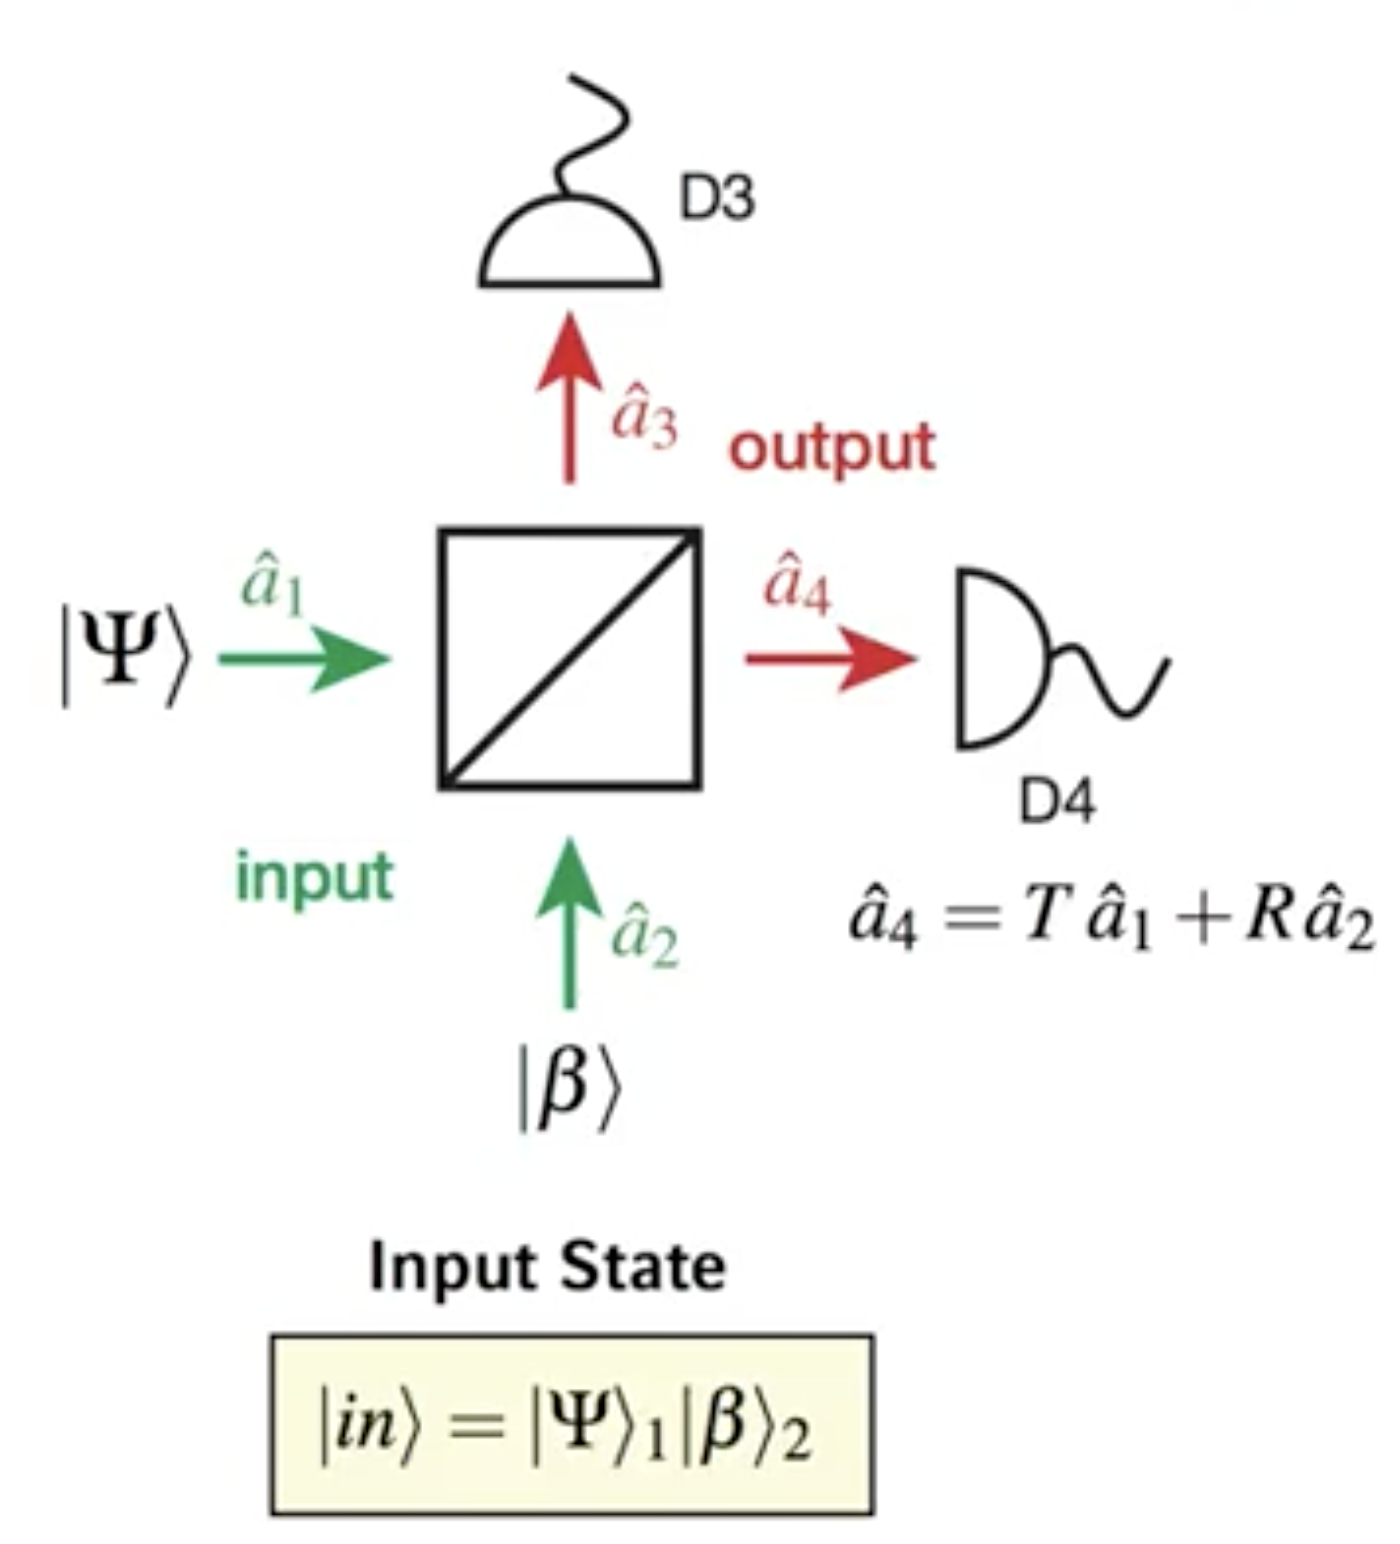
\includegraphics[scale=0.30]{../figures/difference photoncurrent.png}
\begin{proof}
    For a balanced 50/50 beamsplitter, $T = \frac{1}{\sqrt{2}}, R = \frac{1}{\sqrt{2}} i$. Recall that \ref{lemma: creation operators}, $\hat{a}_4 = T \hat{a}_1 + R \hat{a}_2$. We then have
    \begin{align}
        \hat{n}_4
        &= \hat{a}_4^\dagger \hat{a}_4 \\
        &= (T^\ast \hat{a}_1^\dagger + R^\ast \hat{a}_2^\dagger)(T \hat{a}_1 + R \hat{a}_2)\\
        &= (\frac{1}{\sqrt{2}} \hat{a}_1^\dagger - \frac{1}{\sqrt{2}} i \hat{a}_2^\dagger)(\frac{1}{\sqrt{2}} \hat{a}_1 + \frac{1}{\sqrt{2}} i \hat{a}_2) \\
        &= \frac{1}{2} (\hat{a}_1^\dagger - i \hat{a}_2^\dagger)(\hat{a}_1 + i \hat{a}_2) \\
        &= \frac{1}{2}(\hat{a}_1^\dagger \hat{a}_1 - i \hat{a}_2^\dagger \hat{a}_1 + i \hat{a}_1^\dagger \hat{a}_2 + \hat{a}_2^\dagger \hat{a}_2).
    \end{align}
    Similarly, we have
    \begin{align}
        \hat{n}_3 
        &= \hat{a}_3^\dagger \hat{a}_3 \\
        &= \frac{1}{2}(\hat{a}_1^\dagger \hat{a}_1 + i \hat{a}_2^\dagger \hat{a}_1 - i \hat{a}_1^\dagger \hat{a}_2 + \hat{a}_2^\dagger \hat{a}_2).
    \end{align}
    We have $\beta = \vert \beta \vert \exp\left[i \phi\right]$.Then,
    \begin{align}
        i_{34} = i_3 -i_4 \propto \langle in \vert \hat{n}_3 - \hat{n}_4 \vert in \rangle 
        &= -2 _1\langle \Psi \vert _2\langle \beta \vert \frac{1}{2 i} \left(\hat{a}_2^\dagger \hat{a}_1 - \hat{a}_1^\dagger \hat{a}_2\right) \vert \beta \rangle_2 \vert \Psi \rangle_1 \\
        &\qquad\eqnote{To derive the following equation, we need to know that $\hat{a}_1^\dagger, \hat{a}_1$ are applied to $\vert \Psi \rangle_1$ } \nonumber \\
        &\qquad\eqnote{according to its subindex. Similar for subindex 2} \nonumber \\
        &= -2 _1 \langle \Psi \vert \frac{1}{2 i} \left(\beta^\ast \hat{a}_1 - \hat{a}_1^\dagger \beta \right) \vert \Psi \rangle_1 \\
        &=  -2 \vert \beta \vert _1 \langle \Psi \vert \frac{1}{2 i} \left(\hat{a}_1 \exp\left[-i \phi \right] - \hat{a}_1^\dagger \exp\left[i \phi\right] \right) \vert \Psi \rangle_1 \\
        &\qquad\eqnote{By \ref{def: Generalized  quadrature operators}} \nonumber \\
        &= -2 \vert \beta \vert _1\langle \Psi \vert \hat{X}_1(\phi + \frac{\pi}{2}) \vert \Psi \rangle_1, 
    \end{align}
    where $\vert \beta \vert$ is the amplification of quadrature signal.

    \SZQ{$\hat{a}_1^\dagger \hat{a}_2$ must mean $\hat{a}_1^\dagger \otimes \hat{a}_2$. In addition, the order of $\hat{a}_1^\dagger$ and $\hat{a}_2$ needs to be changed according to subindex. These correspondences can be easily understood by the above picture showing the physical setting, where we know that the subindex must coincide.}
\end{proof}


\section{Quantized Light-Atom Interaction}
This section deals with quantized fields and quantized atom.

We have 
\begin{align}
    \hat{H}
    &= \hat{H}_A + \hat{H}_R + \hat{H}_I.
\end{align}

There is a nice picture to show the quantized light field and quantized atom.

Atomic Hamiltonian is 
\begin{align}
    \hat{H}_A
    &= \hbar \omega_{21} \vert 2 \rangle \langle 2 \vert \\
    &= \hbar \omega_{21} \hat{\sigma}^{+} \hat{\sigma}^{-},
\end{align}
where $\hat{\sigma}^{+} = \vert 2 \rangle \langle 1 \vert$ and $\hat{\sigma}^{-} = \vert 1 \rangle \langle 2 \vert$.

Light Hamiltonian is 
\begin{align}
    \hat{H}_R = \sum_{k} \hbar \omega_{k} (\hat{a}^{\dagger}_k \hat{a}_k + \frac{1}{2}).
\end{align}

Light-Atom Interaction Hamiltoniaan is 
\begin{align}
    \hat{H}_I = - \hat{d} \cdot \hat{E}(t).
\end{align}

Rewrite in atomic ladder operators 
\begin{align}
    \hat{d} = e \hat{r} = \hat{\id} \hat{d} \hat{\id} = \sum_{i,j} \vert i \rangle \langle i \vert \hat{d} \vert j \rangle j \vert.
\end{align}
Using parity argument and for the two level system, we have
\begin{align}
    \hat{d} = d_{12} (\hat{\sigma}^{+} + \hat{\sigma}^{-}):= d_{12} (\hat{\sigma}^{\dagger} + \hat{\sigma}).
\end{align}

E-field operator in Schrodinger picture is 
\begin{align}
    \hat{E}(r) = \sum_k \epsilon_k \sqrt{\frac{\hbar \omega_k}{2 \varepsilon_0 V}} \left[\hat{a}_k e^{ikr} + \hat{a}_k^{\dagger} e^{-ikr}\right].
\end{align}
This is a time-independent operator. Then the Interaction Hamiltonian is 
\begin{align}
    \hat{H}_I = \sum_{k} \hbar g_k \left(\hat{a}_k e^{ikr} + \hat{a}^{\dagger}_k e^{-ikr} \right) \left(\hat{\sigma}^{\dagger} + \hat{\sigma}\right),
\end{align}
where $g_k := \sqrt{\frac{\omega_k}{2 \varepsilon_0 \hbar V}} d_{12} \cdot \epsilon_k$ is the light-atom coupling constant (mode-dependent).

Simplified $r = 0$, we have
\begin{align}
    \hat{H}_I = \sum_k \hbar g_k (\hat{a}_k + \hat{a}_k^{\dagger})(\hat{\sigma}^{\dagger} + \hat{\sigma}).
\end{align}
We have four terms: $\hat{a}_k^{\dagger} \hat{\sigma}^{\dagger}$ create atomic excitation and create photon; $\hat{a}_k \hat{\sigma}^{\dagger}$ create atomic excitation and absorpt photon; $\hat{a}_k^{\dagger}\hat{\sigma}$ destroy atomic excitation and emmits photon; $\hat{a}_k \hat{\sigma}$ destroy photon and destroy atomic excitation. $\hat{a}_k^{\dagger} \hat{\sigma}^{\dagger}$ and  $\hat{a}_k \hat{\sigma}$ do not obey energy conservation law, thus are dropped. So we have
\begin{align}
    \hat{H}_I = \sum_{k} \hbar g_k (\underbrace{\hat{a}_k^{\dagger} \hat{\sigma}}_{emission} + \underbrace{\hat{a}_k \hat{\sigma}^{\dagger}}_{absorption}).
\end{align}

Absorption and emission matrix elements. Light field in mode $k$ and atom are described by states
\begin{align}
    \vert n_k, i \rangle = \vert n_k \rangle \otimes \vert i \rangle,
\end{align}
where $\vert n_k \rangle$ is the photon state and $i\vert i \rangle$ is the atomic state. Now, we consider two-level atom. Then we have the absorption of photon from mode $k$ as 
\begin{align}
    \langle n_k -1, 2 \vert \hat{H}_I \vert n_k, 1 \rangle
    &= \hbar g_k \langle n_k -1, 2 \vert {\hat{a}_k^{\dagger} \hat{\sigma}} + {\hat{a}_k \hat{\sigma}^{\dagger}} \vert n_k, 1 \rangle \\
    &= \hbar g_k \sqrt{n_k}.
\end{align} 
We have the emission of photon into mode $k$ as 
\begin{align}
    \langle n_k +1, 1 \vert \hat{H}_I \vert n_k, 2 \rangle
    &= \hbar g_k \langle n_k +1, 1 \vert {\hat{a}_k^{\dagger} \hat{\sigma}} + {\hat{a}_k \hat{\sigma}^{\dagger}} \vert n_k, 2 \rangle \\
    &= \hbar g_k \sqrt{n_k + 1},
\end{align} 
where the $+1$ is surprisingly the \textbf{spontaneous emission}.

\section{Jaynes-Cummings Model} 
Interaction of Time-independent light-atom interaction with single mode of radiation field. Since it is single mode, we drop $k$. The Jaynes-Cummings hamiltonian is
\begin{align}
    \hat{H}_{JC} = \hbar \omega_{21} \hat{\sigma}^{\dagger} \hat{\sigma} + \hbar \omega \hat{a}^\dagger \hat{a} + \hbar g (\hat{a}^{\dagger}\hat{\sigma} + \hat{a}\hat{\sigma}^{\dagger}).
\end{align}

Switch to interaction picture. Interaction hamiltonian in interaction picture is 
\begin{align}
    \hat{H}^{in}_{I}(t) 
    &= e^{\frac{i}{\hbar} \hat{H}_0 t}, \\
    \vert \Psi^{in}(t) \rangle
    &= e^{\frac{i}{\hbar} \hat{H}_0 t \vert \Psi(t) \rangle}.
\end{align}

Interaction Hamiltonian (in interaction picture) is 
\begin{align}
    \hat{H}^{in}_I(t) = \hbar g \left( \hat{a}^{\dagger} \hat{\sigma} e^{i \Delta t} + \hat{a}\hat{\sigma}^{\dagger} e^{- i \Delta t} \right),
\end{align}
where $\Delta = \omega - \omega_{21}$.

Time evolution is 
\begin{align}
    i \hbar \frac{\partial}{\partial t} \vert \Psi^{in}(t) \rangle
    &= \hat{H}^{in}_I(t) \vert \Psi^{in}(t) \rangle.
\end{align}

Assume Ansatz wavefunction 
\begin{align}
    \vert \Psi^{in}(t) \rangle
    &= \sum_n c_{1, n} \vert n, 1 \rangle + c_{2, n} \vert n, 2 \rangle.
\end{align}
\SZQ{Ansatz means "an assumption about the form of an unknown function which is made in order to facilitate solution of an equation or other problem."}

\paragraph*{Time evolution in JC model}
Which states are coupled throught $\hat{H}_I^{in}(t)$?
\begin{align}
    \vert 1, n+1 \rangle  \rightleftarrows_{emission}^{absorption} \vert 2, n \rangle.
\end{align}
Plug the ansatz function into the time evolution equation and have
\begin{align}
    \dot{c}_{1, n+1}(t) 
    &= -i g \sqrt{n+1} e^{+i \Delta t} c_{2, n}(t), \\
    \dot{c}_{2, n}(t) 
    &= -i g \sqrt{n+1} e^{-i \Delta t} c_{1, n+1}(t).
\end{align}

\paragraph*{Time evolution in JC model-solutions}
Initial conditions ($n+1$ photons, atom in ground state) is assumed as
\begin{align}
    c_{1, n+1}(0) = 1.
\end{align}
The resonant interaction $\Delta = 0$. The solution is
\begin{align}
    c_{1, n+1}(t) 
    &= \cos(g\sqrt{n+1} t) \\
    c_{2, n}(t)
    &= -i \sin(g \sqrt{n+1} t).
\end{align}
The corresponding probability is
\begin{align}
    P_{1, n+1}(t) 
    &= \vert c_{1, n+1}(t) \vert^2 = \frac{1}{2} \left[1+\cos(\Omega_n t)\right],
\end{align}
where $\Omega_{n} = 2 g \sqrt{n+1}$ is the quantized rabi frequency. Recall that in the semiclassical case, $\Omega = {d E}/{\hbar}$ is continuous.

Initial conditions (0 photons, atom in excited state) with $n = 0$, $c_{2,0}(0) = 1$ and $\Delta = 0$. The probability is 
\begin{align}
    P_{2, 0}(t)
    &= \vert c_{1, n+1}(t) \vert^2 = \frac{1}{2} \left[1+\cos(\Omega_0 t)\right],
\end{align}
where $\Omega_0 = 2 g$ with vacuum state $n = 0$. There is nice picture showing that state $\vert 2, 0 \rangle$ and $\vert 1, 1 \rangle$ swaps continuously. This is called the Vacuum Rabi-Oscillation! This do not happen in classical case!

\section{Interaction of TLA with a Coherent State}
This section is also called the Collapse and Revival of Rabi Oscillations.

\paragraph*{Time-independent light-atom interaction and coherent state}
The light field is 
\begin{align}
    \vert \alpha \rangle 
    &= e^{-\frac{1}{2}\vert \alpha \vert^2} \sum_{n} \frac{\alpha^n}{\sqrt{n!}} \vert n \rangle.
\end{align}
Assume that atom is initially in excited state $\vert 2 \rangle$. Then for the combined atom-field state amplitudes are 
\begin{align}
    c_{1,n}(0) = 0 \\
    \vert c_{2, n}(0) \vert^2 = e^{\overline{n}} \frac{\overline{n}^n}{n !}.
\end{align}

Recall from the last lecture, we have
\begin{align}
    c_{2,n}(t)
    &= \cos(g \sqrt{n+1} t) \vert c_{2, n}(0) \vert, \\
    c_{1, n}(t)
    &= -i \sin(g \sqrt{n} t) \vert c_{2, n-1}(0) \vert, \forall n \geq 1.
\end{align}
Then inversion is
\begin{align}
    w(t)
    &= P_2(t) - P_1(t) \\
    &= \sum_{n=1}^{\infty} \vert c_{2, n}(t) \vert^2 - \sum_{n=0}^{\infty} \vert c_{1, n}(t) \vert^2 \\
    &= \sum_{n=0}^{\infty} \vert c_{2, n}(0) \vert^2\cos(2 g\sqrt{n+1} t) \\
    &= e^{\overline{n}} \sum_{n=0}^{\infty} \frac{\overline{n}^n}{n!} \cos(2 g \sqrt{n+1} t).
\end{align}
There is a nice picture to plot this inversion for $\overline{n}=20$. Thi shows a Collapse and Revival of Rabi-Oscillations.

\paragraph*{Estimate collapse time}
First, what is collapse time? The collapse time $t_c$ should satisfy
\begin{align}
    \Omega_{\overline{n} + \Delta n} t_c -  \Omega_{\overline{n} - \Delta n} t_c = \pi.
\end{align}
For large $\overline{n}$, we have $\Delta n = \sqrt{\overline{n}}$. We then get
\begin{align}
    (2 g \sqrt{\overline{n} + \sqrt{\overline{n}}} - 2 g \sqrt{\overline{n} - \sqrt{\overline{n}}}) t_c \sim \pi \\
    2 g \left(\sqrt{\overline{n}} \sqrt{1 + \frac{1}{\sqrt{\overline{n}}}} - \sqrt{\overline{n}} \sqrt{1 - \frac{1}{\sqrt{\overline{n}}}} \right) \\
    2 g \left(\sqrt{\overline{n}} {1 + \frac{1}{2}\frac{1}{\sqrt{\overline{n}}}} - \sqrt{\overline{n}} {1 - \frac{1}{2}\frac{1}{\sqrt{\overline{n}}}} \right) \sim \pi.
\end{align}
We have
\begin{align}
    2 g t_c \sim \pi,
\end{align}
so
\begin{align}
    t_c \simeq \frac{\pi}{2 g} = \frac{\pi}{\Omega_0}.
\end{align}
\SZQ{"$\sim$" means asymptotically equal.}

\paragraph{Estimate revival time}
What is revival time? 
\begin{align}
    \Omega_{\overline{n}+1 - \Omega_{\overline{n}}} = 2 \pi.
\end{align}
Revival when 'neighbouring' Rabi Oscillations become in phase! Plug the Rabi frequency, we have
\begin{align}
    &(2 g \sqrt{\overline{n}+1} - 2 g \sqrt{\overline{n}}) t_R \sim 2 \pi \\
    &(2 g \sqrt{\overline{n}} \sqrt{1+\frac{1}{\overline{n}}} - 2 g \sqrt{\overline{n}}) t_R \sim 2 \pi  \\
    &\qquad\eqnote{Using taylor approximation} \\
    &(2 g \sqrt{\overline{n}} (1
    +\frac{1}{2}\frac{1}{\overline{n}})) - 2 g \sqrt{\overline{n}}) t_R \sim 2 \pi  \\
    &(2 g \sqrt{\overline{n}} \frac{1}{2 \sqrt{\overline{n}}}) t_R \sim 2 \pi \\
    &t_R \sim \frac{2 \pi \sqrt{\overline{n}}}{g} = \frac{4 \pi \sqrt{\overline{n}}}{\Omega_0}.
\end{align}

\paragraph*{Classical limit}
Quantized box $V \rightarrow \infty$, then $g \rightarrow 0$.

Keep Rabi frequency constant by $g \rightarrow 0, \overline{n} \rightarrow \infty$, which means 
\begin{align}
    2 g \sqrt{\overline{n}} = \Omega = constant \\
    t_c \sim \frac{\pi}{2 g} \rightarrow \infty, for~g \rightarrow 0.
\end{align}
This means collapse becomes absent.

There is a nice experiment of the test of quantized Rabi Oscillations.

\section{Primer on Cavity Quantum Electrodynamics}
This section provides the experimental setup and results for the quantized light-atom interaction. There are many pictures reffering to the video.

How can we experimentally observe quantized light-atom interaction?
\begin{align}
    \hat{H}_I = \hbar g(\hat{a}^{\dagger} \hat{\sigma} + \hat{a} \hat{\sigma}^{\dagger}), \\
    g = \sqrt{\frac{\hbar \omega}{2 \varepsilon_0 V}} d_{12} \cdot \epsilon.
\end{align}
$V$ small! Use cavity!! 

\paragraph*{Light field cavity}
finite reflectivity.

$k$: transmission losses of cavity (finite reflectivity mirrors).

$\gamma$: spontaneous emission of atom into free space.

$g$: coherent coupling.

$k, \gamma$: incoherent dynamics.

$g$: coherent dynamics.

Define $C := \frac{g^2}{k \gamma}$ cooperativity.

\paragraph*{Experimentally used CQED Setups}
1) Superconducting mirrors for photons in microwave regime (Haroche, Walter)

3) On-chip mitrowaave resonators with superconducting qubits (Schoelkopf, Matinis, Wallraff) 

Details ref to the video.

\paragraph*{Rydberg atoms}
$d_{12}$ large.

Energy spectrum
\begin{align}
    E_{n,l} = - \frac{R}{(n-\delta_{l})^2} = \simeq - \frac{R}{n^2}.
\end{align}

Huge dipole moment
\begin{align}
    \langle \phi_{n, l^{\prime}} \vert q \hat{r} \vert \phi_{n, l} \rangle \simeq q a_0 n^2.
\end{align}

\section{Seeing a Single Photon without Destroying it}
\paragraph*{Detecting a photon with photondetector}
Usually through absorption: single photon $\rightarrow$ photodetector.

Can we detect a photon without destroying it ???

Yes! interferometrically. Experimental setup: ref to video.

Step 1: $\pi/2$ pulse in Ramsey Zone 1 (on i-g transition)

Step 2: a) if 1 photon in cavity $\vert g, 1 \rangle \rightarrow e^{i \pi} \vert g, 1 \rangle = - \vert g, 1\rangle$. $2 g t_{int} = 2 \pi$. b) if 0 photons in cavity $\vert g, 0 \rangle \rightarrow \vert g, 0 \rangle$.

Step 3: $\pi/2$ pulse in Ramsey Zone 2 (on i-g transition)

There are nice pictures about the experimental results.

\section{Dressed States}
\paragraph*{Atom-light field without interaction}
Atom: $\hat{H}_A = \hbar \omega_{21} \hat{\sigma}^{\dagger} \hat{\sigma}$.

Fight field: $\hat{H}_L = \hbar \omega \hat{a}^{\dagger} \hat{a}$.

\paragraph{Atom-light field}
Group the eigenstates: $\vert 1, n+2 \rangle, \vert 2, n+1 \rangle$, $\vert 1, n+1 \rangle, \vert 2, n \rangle$, $\vert 1, n \rangle, \vert 2, n-1 \rangle$.

\paragraph*{Dressed states}
$\hat{H}_A + \hat{H}_R$ eigenstates of uncoupled hamiltonian $\vert 1, n+1 \rangle, \vert 2, n \rangle$ $\rightleftarrows$ $\vert 1(n) \rangle, \vert 2(n) \rangle$ $\hat{H}_A + \hat{H}_R + \hat{H}_I$ eigenstates of coupled hamiltonian.

Dressed state eigenstates
\begin{align}
    \vert 1(n) \rangle = \sin(\theta/2) \vert 1, n+1 \rangle + \cos(\theta/2) \vert 2, n \rangle \\
    \vert 2(n) \rangle = \cos(\theta/2) \vert 1, n+1 \rangle - \sin(\theta/2) \vert 2, n \rangle,
\end{align}
where $\tan \theta = -\Omega_n/\Delta$, $\sin(\theta/2) = \sqrt{\frac{\Omega_n^{\Delta} - \Delta}{2 \Omega_n^{\Delta}}}$, $\cos(\theta/2) = \sqrt{\frac{\Omega_n^{\Delta} + \Delta}{2 \Omega_n^{\Delta}}}$ and the generalized Rabi frequency is $\Omega_{n}^{\Delta} = \sqrt{\Omega_n^2 + \Delta^2}$, $\Omega_n = 2g \sqrt{n+1}$.

There is a nice picture.

\paragraph*{Avoided corssing of energy levels}
There is a nice picture.

Dressed state for $\Delta = 0 \rightarrow \theta = \pi/2$, we have
\begin{align}
    \vert 1(n) \rangle =  \frac{1}{\sqrt{2}}(\vert 1, n+1 \rangle + \vert 2, n \rangle)\\
    \vert 2(n) \rangle =  \frac{1}{\sqrt{2}}(\vert 1, n+1 \rangle - \vert 2, n \rangle).
\end{align}

\paragraph*{Re-interpreting Rabi Oscillations}
Initial state
\begin{align}
    \vert \Psi(0) \rangle = \vert 1, n+1 \rangle 
    &= \frac{1}{\sqrt{2}} (\vert 1(n) \rangle + \vert 2(n) \rangle) \\
    \vert \psi(t) \rangle = \frac{1}{\sqrt{2}} (e^{i \Omega_n t} \vert 1(n) \rangle + \vert 2(n) \rangle). \\
    P_1(t) 
    &= \vert \langle 1, n+1 \vert \psi(t) \rangle\vert^2 \\
    &= \frac{1}{2}\vert \frac{1}{\sqrt{2}} e^{-i \Omega_n t} + \frac{1}{\sqrt{2}} \vert^2 \\
    &= \frac{1}{4} \vert e^{-i \Omega_n t} + 1 \vert^2 \\
    &= \frac{1}{4} \vert e^{-i \Omega_n t/2} + e^{i \Omega_n t/2} \vert^2 \\
    &= \cos^2(\Omega_n t/2).
\end{align}



\end{document}